% lecture5_ro.tex -- GENERATED by build_L5.py from L5_numbers.json; do not edit by hand.
\documentclass[10pt,aspectratio=169,t]{beamer}
% =============================================================================
% nn_preamble.tex -- shared Beamer preamble of Neural Networks and Deep Learning (NN)
% Used by every lecture: lectures/Lk/lecturek.tex does
%   \documentclass[10pt,aspectratio=169,t]{beamer}
%   % =============================================================================
% nn_preamble.tex -- shared Beamer preamble of Neural Networks and Deep Learning (NN)
% Used by every lecture: lectures/Lk/lecturek.tex does
%   \documentclass[10pt,aspectratio=169,t]{beamer}
%   % =============================================================================
% nn_preamble.tex -- shared Beamer preamble of Neural Networks and Deep Learning (NN)
% Used by every lecture: lectures/Lk/lecturek.tex does
%   \documentclass[10pt,aspectratio=169,t]{beamer}
%   \input{../common/nn_preamble}
%   \nnlecture{k}{Lecture title}
% Logos live in lectures/common/logos/, charts in lectures/Lk/charts/.
% Do NOT add \hfuzz / \vfuzz / \hbadness here: overfull boxes must be fixed, not hidden.
% =============================================================================

\usetheme{default}
\setbeamersize{text margin left=7mm, text margin right=7mm}

% ---------------------------------------------------------------- packages
\usepackage[utf8]{inputenc}
\usepackage[T1]{fontenc}
\usepackage{lmodern}
\usepackage{amsmath, amssymb}
\usepackage{mathtools}
\usepackage{bm}
\usepackage{tikz}
\usetikzlibrary{arrows.meta, positioning, calc, shapes.misc}
\usepackage{booktabs}
\usepackage{array}
\usepackage{graphicx}
\usepackage{colortbl}
\usepackage{xcolor}
\usepackage{multicol}
\hypersetup{colorlinks=true, linkcolor=MainBlue, urlcolor=MainBlue, citecolor=MainBlue}
\graphicspath{{../common/logos/}}   % charts are included with their language folder: charts/en/, charts/ro/

% ---------------------------------------------------------------- colours
\definecolor{MainBlue}{RGB}{26, 58, 110}
\definecolor{IDAred}{RGB}{205, 0, 0}
\definecolor{DarkGray}{RGB}{51, 51, 51}
\definecolor{FooterGray}{RGB}{100, 100, 100}
\definecolor{BlockGray}{RGB}{236, 238, 242}
\definecolor{KeynoteGray}{RGB}{218, 218, 218}
\definecolor{Crimson}{RGB}{190, 40, 50}
\definecolor{Forest}{RGB}{30, 110, 50}
\definecolor{Bitter}{RGB}{214, 150, 20}
% chart palette (same hex values and order as lectures/common/nn_plot.py SERIES)
\definecolor{Ser1}{HTML}{2A78D6}
\definecolor{Ser2}{HTML}{EB6834}
\definecolor{Ser3}{HTML}{1BAF7A}
\definecolor{Ser4}{HTML}{EDA100}
\definecolor{Ser5}{HTML}{E87BA4}
\definecolor{Ser6}{HTML}{008300}
\definecolor{Ser7}{HTML}{6250D6}
\definecolor{Ser8}{HTML}{E34948}

\setbeamertemplate{background}{%
  \begin{tikzpicture}[remember picture, overlay]
    \shade[shading=axis, shading angle=315, top color=white, bottom color=KeynoteGray]
      (current page.south west) rectangle (current page.north east);
  \end{tikzpicture}}
\setbeamercolor{background canvas}{bg=}
\setbeamercolor{structure}{fg=MainBlue}
\setbeamercolor{normal text}{fg=DarkGray}
\setbeamercolor{title}{fg=IDAred}
\setbeamercolor{frametitle}{fg=IDAred, bg=}
\setbeamercolor{block title}{bg=MainBlue, fg=white}
\setbeamercolor{block body}{bg=BlockGray, fg=DarkGray}
\setbeamercolor{block title alerted}{bg=Crimson, fg=white}
\setbeamercolor{block body alerted}{bg=Crimson!7, fg=DarkGray}
\setbeamercolor{block title example}{bg=Forest, fg=white}
\setbeamercolor{block body example}{bg=Forest!7, fg=DarkGray}
\setbeamercolor{item}{fg=MainBlue}
\setbeamerfont{frametitle}{size=\large, series=\bfseries}
\setbeamerfont{block title}{size=\small, series=\bfseries}
\setbeamertemplate{blocks}[rounded][shadow=false]
\setbeamertemplate{itemize item}{\color{MainBlue}$\boxdot$}
\setbeamertemplate{itemize subitem}{\color{MainBlue}\scriptsize$\blacktriangleright$}
% compact two-level lists: level 1 = main point, level 2 = details (no text outside bullets)
\setbeamerfont{itemize/enumerate subbody}{size=\footnotesize}
\setlength{\leftmargini}{1.1em}
\setlength{\leftmarginii}{1.1em}
\setbeamertemplate{itemize/enumerate body begin}{\setlength{\topsep}{0pt}\setlength{\partopsep}{0pt}\setlength{\parskip}{0pt}}
\setbeamertemplate{itemize/enumerate subbody begin}{\setlength{\topsep}{0pt}\setlength{\partopsep}{0pt}\setlength{\itemsep}{0pt}\vspace{-0.4ex}}

\setbeamertemplate{enumerate item}{\color{MainBlue}\insertenumlabel.}
\setlength{\leftmargini}{1.3em}
\setlength{\leftmarginii}{1.2em}
\setbeamertemplate{navigation symbols}{}
\setbeamertemplate{section in toc}{\color{MainBlue}$\blacktriangleright$~\inserttocsection}
\setbeamertemplate{caption}{\raggedright\insertcaption\par}
% frame subtitle = precise citation line under the claim title (Weron style)
\setbeamerfont{framesubtitle}{size=\footnotesize}
\setbeamercolor{framesubtitle}{fg=FooterGray}
% outline that reappears at every section with the current section highlighted
\setbeamertemplate{section in toc shaded}[default][35]
\setbeamertemplate{subsection in toc shaded}[default][35]
\setbeamertemplate{subsection in toc}{\leavevmode\leftskip=2.2em\color{DarkGray}\small\inserttocsubsection\par}
\AtBeginSection[]{{\begin{frame}{\txtoutline}\vspace{2mm}\small
  \tableofcontents[currentsection,hideothersubsections]\end{frame}}}

% ---------------------------------------------------------------- head and foot
\setbeamertemplate{headline}{%
  \vskip10pt%
  \hbox to \paperwidth{\hskip0.5cm%
    {\small\color{FooterGray}\renewcommand{\hyperlink}[2]{##2}\insertsectionhead}%
    \hfill\textcolor{FooterGray}{\small\insertframenumber}\hskip0.5cm}%
  \vskip4pt{\color{FooterGray}\hrule height 0.4pt}}
% footer as in the other courses (MFM, SFM): course name on the left, small sparkline on the right
\setbeamertemplate{footline}{%
  {\color{FooterGray}\hrule height 0.4pt}\vskip4pt%
  \hbox to \paperwidth{\hskip0.5cm%
    \textcolor{FooterGray}{\small\txtcourse}%
    \hfill\raisebox{-0.1em}{\begin{tikzpicture}[x=0.08em, y=0.08em, line width=0.4pt]
      \draw[FooterGray] (0,3) -- (1,4) -- (2,3.5) -- (3,5) -- (4,4) -- (5,6) -- (6,5.5) -- (7,4) -- (8,5) -- (9,7) -- (10,6) -- (11,5) -- (12,6.5) -- (13,8) -- (14,7) -- (15,6) -- (16,7.5) -- (17,9) -- (18,8) -- (19,7) -- (20,8.5) -- (21,10) -- (22,9) -- (23,8) -- (24,9.5);
    \end{tikzpicture}}\hskip0.5cm}%
  \vskip6pt}

% ---------------------------------------------------------------- title page
\defbeamertemplate*{title page}{nn}[1][]{%
  \vspace{0.15cm}
  \begin{center}
    \href{https://www.ase.ro}{
\includegraphics[height=0.9cm]{ase_logo.png}}\hspace{0.3cm}%
    \href{https://ipe.ro/new}{
\includegraphics[height=0.9cm]{acad_logo.png}}\hspace{0.3cm}%
    \href{https://theida.net}{
\includegraphics[height=0.9cm]{ida_logo.png}}\hspace{0.3cm}%
    \href{https://blockchain-research-center.com}{
\includegraphics[height=0.9cm]{brc_logo.png}}\hspace{0.3cm}%
    \href{https://www.ai4efin.ase.ro}{
\includegraphics[height=0.9cm]{ai4efin_logo.png}}\hspace{0.3cm}%
    \href{https://www.digital-finance-msca.com}{
\includegraphics[height=0.9cm]{msca_logo.png}}%
  \end{center}
  \vspace{0.45cm}
  \begin{center}
    \begin{minipage}{0.1\textwidth}\centering
      \href{https://quantlet.com}{
\includegraphics[height=0.9cm]{ql_logo.png}}\end{minipage}%
    \begin{minipage}{0.78\textwidth}\centering
      {\Large\bfseries\usebeamercolor[fg]{title}\inserttitle}\par\vspace{0.25cm}
      {\large\usebeamercolor[fg]{title}\insertsubtitle}\end{minipage}%
    \begin{minipage}{0.1\textwidth}\centering
      \href{https://quantinar.com}{
\includegraphics[height=0.9cm]{qr_logo.png}}\end{minipage}
  \end{center}
  \vfill
  \hspace{0.4cm}{\bfseries\insertauthor}\par\vspace{0.12cm}
  \hspace{0.4cm}\begin{minipage}[t]{0.92\textwidth}\raggedright\footnotesize\insertinstitute\end{minipage}
  \par\vspace{0.4cm}}

% ---------------------------------------------------------------- lecture metadata
\newcommand{\nnshort}{}
\newcommand{\nnnb}{notebooks}
\newcommand{\nnrepo}{https://github.com/danpele/NEURAL_BIZ/tree/main}
% language-dependent labels (English default; \nnromanian switches to Romanian, call it before \nnlecture)
\newcommand{\txtcourse}{Neural Networks and Deep Learning}
\newcommand{\txtlecture}{Lecture}
\newcommand{\txtoutline}{Outline}
\newcommand{\txtintuition}{In one sentence:}
\newcommand{\txtjob}{In practice:}
\newcommand{\txttry}{Experiment yourself:}
\newcommand{\txtwhere}{where}
\newcommand{\txtsim}{SIMULATED DATA (teaching illustration)}
\newcommand{\txtnbsuffix}{}
\newcommand{\txtinstitute}{Bucharest University of Economic Studies (ASE), Department of Statistics and Econometrics\\
    Romanian Academy, Institute for Economic Forecasting (IPE)\\
    IDA Institute Digital Assets \textbullet\ AI4EFin \textbullet\ MSCA Digital Finance}
\newcommand{\nnromanian}{%
  \renewcommand{\txtcourse}{Rețele neuronale și deep learning}%
  \renewcommand{\txtlecture}{Cursul}%
  \renewcommand{\txtoutline}{Cuprins}%
  \renewcommand{\txtintuition}{Pe scurt:}%
  \renewcommand{\txtjob}{În practică:}%
  \renewcommand{\txttry}{Exercițiu practic:}%
  \renewcommand{\txtwhere}{unde}%
  \renewcommand{\txtsim}{DATE SIMULATE (doar pentru ilustrare)}%
  \renewcommand{\txtnbsuffix}{\string_ro}%
  \renewcommand{\txtinstitute}{Academia de Studii Economice din București (ASE), Departamentul de Statistică și Econometrie\\
    Academia Română, Institutul de Prognoză Economică (IPE)\\
    IDA Institute Digital Assets \textbullet\ AI4EFin \textbullet\ MSCA Digital Finance}}
\newcommand{\nnlecture}[2]{%
  \renewcommand{\nnshort}{\txtlecture\ #1}%
  \renewcommand{\nnnb}{notebooks/L#1\string_notebook\txtnbsuffix.ipynb}%
  \title[NN]{\txtcourse}%
  \subtitle{\txtlecture\ #1: #2}%
  \author{Prof.\ dr.\ Daniel Traian PELE}%
  \institute{\txtinstitute}%
  \date{}}

% ---------------------------------------------------------------- teaching blocks (one message per frame)
% \intuition{one plain sentence}  ->  formula with every symbol defined  ->  real-data example  ->  \manager{one line}
\newcommand{\intuition}[1]{\begin{itemize}\item {\color{MainBlue}\textbf{\txtintuition}}~#1\end{itemize}\vspace{0.6mm}}
\newcommand{\manager}[1]{\colorbox{Forest!10}{\parbox{\dimexpr\linewidth-2\fboxsep\relax}{\footnotesize
  \begin{itemize}\setlength{\itemsep}{0pt}\item \textbf{\color{Forest}\txtjob}~#1\end{itemize}}}}
% Experiment yourself: pointer to the matching notebook section
\newcommand{\tryit}[1]{{\scriptsize\href{\nnrepo/\nnnb}{%
  \raisebox{-0.15em}{
\includegraphics[height=0.85em]{ql_logo.png}}\,\textbf{\txttry}~\color{MainBlue}#1}}}
% bottom row: manager line (left) + experiment pointer (right), pinned to the bottom of the frame
\newcommand{\bottomrow}[2]{\par\vfill\noindent\begin{minipage}[b]{0.72\linewidth}#1\end{minipage}\hfill
  \begin{minipage}[b]{0.26\linewidth}\raggedleft #2\end{minipage}\par\vspace{0.5mm}}
\newcommand{\where}[1]{{\footnotesize\textbf{\txtwhere}~#1\par}}

% ---------------------------------------------------------------- helpers
% chart source line under a figure: \chartsource{Source ...; period ...}
\newcommand{\chartsource}[1]{\par\vspace{1pt}{\scriptsize\color{FooterGray}#1\par}}
% link to code: \quantlet{label}{path inside the repo}
\newcommand{\quantlet}[2]{\par\vspace{1pt}\hfill\href{\nnrepo/#2}{%
  \raisebox{-0.15em}{
\includegraphics[height=0.75em]{ql_logo.png}}\textcolor{MainBlue}{\scriptsize\ #1}}}
% inline Quantlet link for the bottom-right corner of a frame: \qlink{label}{path inside the repo}
\newcommand{\qlink}[2]{{\scriptsize\href{\nnrepo/#2}{\raisebox{-0.15em}{
\includegraphics[height=0.85em]{ql_logo.png}}\,\textcolor{MainBlue}{#1}}}}
\newcommand{\simlabel}{\colorbox{Crimson!12}{\scriptsize\bfseries\color{Crimson}\txtsim}}
\newcommand{\E}{\mathbb{E}}
\newcommand{\Var}{\operatorname{Var}}
\newcommand{\Cov}{\operatorname{Cov}}
\newcommand{\Corr}{\operatorname{Corr}}
\newcommand{\asinh}{\operatorname{asinh}}
\newcommand{\iid}{\overset{\text{i.i.d.}}{\sim}}
\newcommand{\EUR}{EUR}
% deep-learning notation (Bishop & Bishop, 2024): vectors bold lower case, matrices bold upper case
\newcommand{\R}{\mathbb{R}}
\newcommand{\vx}{\mathbf{x}}
\newcommand{\vy}{\mathbf{y}}
\newcommand{\vz}{\mathbf{z}}
\newcommand{\vh}{\mathbf{h}}
\newcommand{\vw}{\mathbf{w}}
\newcommand{\vb}{\mathbf{b}}
\newcommand{\mW}{\mathbf{W}}
\newcommand{\mX}{\mathbf{X}}
\newcommand{\btheta}{\boldsymbol{\theta}}
\newcommand{\loss}{\mathcal{L}}
\newcommand{\dataset}{\mathcal{D}}
\DeclareMathOperator*{\argmin}{arg\,min}
\DeclareMathOperator*{\argmax}{arg\,max}
\DeclareMathOperator{\softmax}{softmax}
\DeclareMathOperator{\ReLU}{ReLU}
\DeclareMathOperator{\sigm}{\sigma}

%   \nnlecture{k}{Lecture title}
% Logos live in lectures/common/logos/, charts in lectures/Lk/charts/.
% Do NOT add \hfuzz / \vfuzz / \hbadness here: overfull boxes must be fixed, not hidden.
% =============================================================================

\usetheme{default}
\setbeamersize{text margin left=7mm, text margin right=7mm}

% ---------------------------------------------------------------- packages
\usepackage[utf8]{inputenc}
\usepackage[T1]{fontenc}
\usepackage{lmodern}
\usepackage{amsmath, amssymb}
\usepackage{mathtools}
\usepackage{bm}
\usepackage{tikz}
\usetikzlibrary{arrows.meta, positioning, calc, shapes.misc}
\usepackage{booktabs}
\usepackage{array}
\usepackage{graphicx}
\usepackage{colortbl}
\usepackage{xcolor}
\usepackage{multicol}
\hypersetup{colorlinks=true, linkcolor=MainBlue, urlcolor=MainBlue, citecolor=MainBlue}
\graphicspath{{../common/logos/}}   % charts are included with their language folder: charts/en/, charts/ro/

% ---------------------------------------------------------------- colours
\definecolor{MainBlue}{RGB}{26, 58, 110}
\definecolor{IDAred}{RGB}{205, 0, 0}
\definecolor{DarkGray}{RGB}{51, 51, 51}
\definecolor{FooterGray}{RGB}{100, 100, 100}
\definecolor{BlockGray}{RGB}{236, 238, 242}
\definecolor{KeynoteGray}{RGB}{218, 218, 218}
\definecolor{Crimson}{RGB}{190, 40, 50}
\definecolor{Forest}{RGB}{30, 110, 50}
\definecolor{Bitter}{RGB}{214, 150, 20}
% chart palette (same hex values and order as lectures/common/nn_plot.py SERIES)
\definecolor{Ser1}{HTML}{2A78D6}
\definecolor{Ser2}{HTML}{EB6834}
\definecolor{Ser3}{HTML}{1BAF7A}
\definecolor{Ser4}{HTML}{EDA100}
\definecolor{Ser5}{HTML}{E87BA4}
\definecolor{Ser6}{HTML}{008300}
\definecolor{Ser7}{HTML}{6250D6}
\definecolor{Ser8}{HTML}{E34948}

\setbeamertemplate{background}{%
  \begin{tikzpicture}[remember picture, overlay]
    \shade[shading=axis, shading angle=315, top color=white, bottom color=KeynoteGray]
      (current page.south west) rectangle (current page.north east);
  \end{tikzpicture}}
\setbeamercolor{background canvas}{bg=}
\setbeamercolor{structure}{fg=MainBlue}
\setbeamercolor{normal text}{fg=DarkGray}
\setbeamercolor{title}{fg=IDAred}
\setbeamercolor{frametitle}{fg=IDAred, bg=}
\setbeamercolor{block title}{bg=MainBlue, fg=white}
\setbeamercolor{block body}{bg=BlockGray, fg=DarkGray}
\setbeamercolor{block title alerted}{bg=Crimson, fg=white}
\setbeamercolor{block body alerted}{bg=Crimson!7, fg=DarkGray}
\setbeamercolor{block title example}{bg=Forest, fg=white}
\setbeamercolor{block body example}{bg=Forest!7, fg=DarkGray}
\setbeamercolor{item}{fg=MainBlue}
\setbeamerfont{frametitle}{size=\large, series=\bfseries}
\setbeamerfont{block title}{size=\small, series=\bfseries}
\setbeamertemplate{blocks}[rounded][shadow=false]
\setbeamertemplate{itemize item}{\color{MainBlue}$\boxdot$}
\setbeamertemplate{itemize subitem}{\color{MainBlue}\scriptsize$\blacktriangleright$}
% compact two-level lists: level 1 = main point, level 2 = details (no text outside bullets)
\setbeamerfont{itemize/enumerate subbody}{size=\footnotesize}
\setlength{\leftmargini}{1.1em}
\setlength{\leftmarginii}{1.1em}
\setbeamertemplate{itemize/enumerate body begin}{\setlength{\topsep}{0pt}\setlength{\partopsep}{0pt}\setlength{\parskip}{0pt}}
\setbeamertemplate{itemize/enumerate subbody begin}{\setlength{\topsep}{0pt}\setlength{\partopsep}{0pt}\setlength{\itemsep}{0pt}\vspace{-0.4ex}}

\setbeamertemplate{enumerate item}{\color{MainBlue}\insertenumlabel.}
\setlength{\leftmargini}{1.3em}
\setlength{\leftmarginii}{1.2em}
\setbeamertemplate{navigation symbols}{}
\setbeamertemplate{section in toc}{\color{MainBlue}$\blacktriangleright$~\inserttocsection}
\setbeamertemplate{caption}{\raggedright\insertcaption\par}
% frame subtitle = precise citation line under the claim title (Weron style)
\setbeamerfont{framesubtitle}{size=\footnotesize}
\setbeamercolor{framesubtitle}{fg=FooterGray}
% outline that reappears at every section with the current section highlighted
\setbeamertemplate{section in toc shaded}[default][35]
\setbeamertemplate{subsection in toc shaded}[default][35]
\setbeamertemplate{subsection in toc}{\leavevmode\leftskip=2.2em\color{DarkGray}\small\inserttocsubsection\par}
\AtBeginSection[]{{\begin{frame}{\txtoutline}\vspace{2mm}\small
  \tableofcontents[currentsection,hideothersubsections]\end{frame}}}

% ---------------------------------------------------------------- head and foot
\setbeamertemplate{headline}{%
  \vskip10pt%
  \hbox to \paperwidth{\hskip0.5cm%
    {\small\color{FooterGray}\renewcommand{\hyperlink}[2]{##2}\insertsectionhead}%
    \hfill\textcolor{FooterGray}{\small\insertframenumber}\hskip0.5cm}%
  \vskip4pt{\color{FooterGray}\hrule height 0.4pt}}
% footer as in the other courses (MFM, SFM): course name on the left, small sparkline on the right
\setbeamertemplate{footline}{%
  {\color{FooterGray}\hrule height 0.4pt}\vskip4pt%
  \hbox to \paperwidth{\hskip0.5cm%
    \textcolor{FooterGray}{\small\txtcourse}%
    \hfill\raisebox{-0.1em}{\begin{tikzpicture}[x=0.08em, y=0.08em, line width=0.4pt]
      \draw[FooterGray] (0,3) -- (1,4) -- (2,3.5) -- (3,5) -- (4,4) -- (5,6) -- (6,5.5) -- (7,4) -- (8,5) -- (9,7) -- (10,6) -- (11,5) -- (12,6.5) -- (13,8) -- (14,7) -- (15,6) -- (16,7.5) -- (17,9) -- (18,8) -- (19,7) -- (20,8.5) -- (21,10) -- (22,9) -- (23,8) -- (24,9.5);
    \end{tikzpicture}}\hskip0.5cm}%
  \vskip6pt}

% ---------------------------------------------------------------- title page
\defbeamertemplate*{title page}{nn}[1][]{%
  \vspace{0.15cm}
  \begin{center}
    \href{https://www.ase.ro}{
\includegraphics[height=0.9cm]{ase_logo.png}}\hspace{0.3cm}%
    \href{https://ipe.ro/new}{
\includegraphics[height=0.9cm]{acad_logo.png}}\hspace{0.3cm}%
    \href{https://theida.net}{
\includegraphics[height=0.9cm]{ida_logo.png}}\hspace{0.3cm}%
    \href{https://blockchain-research-center.com}{
\includegraphics[height=0.9cm]{brc_logo.png}}\hspace{0.3cm}%
    \href{https://www.ai4efin.ase.ro}{
\includegraphics[height=0.9cm]{ai4efin_logo.png}}\hspace{0.3cm}%
    \href{https://www.digital-finance-msca.com}{
\includegraphics[height=0.9cm]{msca_logo.png}}%
  \end{center}
  \vspace{0.45cm}
  \begin{center}
    \begin{minipage}{0.1\textwidth}\centering
      \href{https://quantlet.com}{
\includegraphics[height=0.9cm]{ql_logo.png}}\end{minipage}%
    \begin{minipage}{0.78\textwidth}\centering
      {\Large\bfseries\usebeamercolor[fg]{title}\inserttitle}\par\vspace{0.25cm}
      {\large\usebeamercolor[fg]{title}\insertsubtitle}\end{minipage}%
    \begin{minipage}{0.1\textwidth}\centering
      \href{https://quantinar.com}{
\includegraphics[height=0.9cm]{qr_logo.png}}\end{minipage}
  \end{center}
  \vfill
  \hspace{0.4cm}{\bfseries\insertauthor}\par\vspace{0.12cm}
  \hspace{0.4cm}\begin{minipage}[t]{0.92\textwidth}\raggedright\footnotesize\insertinstitute\end{minipage}
  \par\vspace{0.4cm}}

% ---------------------------------------------------------------- lecture metadata
\newcommand{\nnshort}{}
\newcommand{\nnnb}{notebooks}
\newcommand{\nnrepo}{https://github.com/danpele/NEURAL_BIZ/tree/main}
% language-dependent labels (English default; \nnromanian switches to Romanian, call it before \nnlecture)
\newcommand{\txtcourse}{Neural Networks and Deep Learning}
\newcommand{\txtlecture}{Lecture}
\newcommand{\txtoutline}{Outline}
\newcommand{\txtintuition}{In one sentence:}
\newcommand{\txtjob}{In practice:}
\newcommand{\txttry}{Experiment yourself:}
\newcommand{\txtwhere}{where}
\newcommand{\txtsim}{SIMULATED DATA (teaching illustration)}
\newcommand{\txtnbsuffix}{}
\newcommand{\txtinstitute}{Bucharest University of Economic Studies (ASE), Department of Statistics and Econometrics\\
    Romanian Academy, Institute for Economic Forecasting (IPE)\\
    IDA Institute Digital Assets \textbullet\ AI4EFin \textbullet\ MSCA Digital Finance}
\newcommand{\nnromanian}{%
  \renewcommand{\txtcourse}{Rețele neuronale și deep learning}%
  \renewcommand{\txtlecture}{Cursul}%
  \renewcommand{\txtoutline}{Cuprins}%
  \renewcommand{\txtintuition}{Pe scurt:}%
  \renewcommand{\txtjob}{În practică:}%
  \renewcommand{\txttry}{Exercițiu practic:}%
  \renewcommand{\txtwhere}{unde}%
  \renewcommand{\txtsim}{DATE SIMULATE (doar pentru ilustrare)}%
  \renewcommand{\txtnbsuffix}{\string_ro}%
  \renewcommand{\txtinstitute}{Academia de Studii Economice din București (ASE), Departamentul de Statistică și Econometrie\\
    Academia Română, Institutul de Prognoză Economică (IPE)\\
    IDA Institute Digital Assets \textbullet\ AI4EFin \textbullet\ MSCA Digital Finance}}
\newcommand{\nnlecture}[2]{%
  \renewcommand{\nnshort}{\txtlecture\ #1}%
  \renewcommand{\nnnb}{notebooks/L#1\string_notebook\txtnbsuffix.ipynb}%
  \title[NN]{\txtcourse}%
  \subtitle{\txtlecture\ #1: #2}%
  \author{Prof.\ dr.\ Daniel Traian PELE}%
  \institute{\txtinstitute}%
  \date{}}

% ---------------------------------------------------------------- teaching blocks (one message per frame)
% \intuition{one plain sentence}  ->  formula with every symbol defined  ->  real-data example  ->  \manager{one line}
\newcommand{\intuition}[1]{\begin{itemize}\item {\color{MainBlue}\textbf{\txtintuition}}~#1\end{itemize}\vspace{0.6mm}}
\newcommand{\manager}[1]{\colorbox{Forest!10}{\parbox{\dimexpr\linewidth-2\fboxsep\relax}{\footnotesize
  \begin{itemize}\setlength{\itemsep}{0pt}\item \textbf{\color{Forest}\txtjob}~#1\end{itemize}}}}
% Experiment yourself: pointer to the matching notebook section
\newcommand{\tryit}[1]{{\scriptsize\href{\nnrepo/\nnnb}{%
  \raisebox{-0.15em}{
\includegraphics[height=0.85em]{ql_logo.png}}\,\textbf{\txttry}~\color{MainBlue}#1}}}
% bottom row: manager line (left) + experiment pointer (right), pinned to the bottom of the frame
\newcommand{\bottomrow}[2]{\par\vfill\noindent\begin{minipage}[b]{0.72\linewidth}#1\end{minipage}\hfill
  \begin{minipage}[b]{0.26\linewidth}\raggedleft #2\end{minipage}\par\vspace{0.5mm}}
\newcommand{\where}[1]{{\footnotesize\textbf{\txtwhere}~#1\par}}

% ---------------------------------------------------------------- helpers
% chart source line under a figure: \chartsource{Source ...; period ...}
\newcommand{\chartsource}[1]{\par\vspace{1pt}{\scriptsize\color{FooterGray}#1\par}}
% link to code: \quantlet{label}{path inside the repo}
\newcommand{\quantlet}[2]{\par\vspace{1pt}\hfill\href{\nnrepo/#2}{%
  \raisebox{-0.15em}{
\includegraphics[height=0.75em]{ql_logo.png}}\textcolor{MainBlue}{\scriptsize\ #1}}}
% inline Quantlet link for the bottom-right corner of a frame: \qlink{label}{path inside the repo}
\newcommand{\qlink}[2]{{\scriptsize\href{\nnrepo/#2}{\raisebox{-0.15em}{
\includegraphics[height=0.85em]{ql_logo.png}}\,\textcolor{MainBlue}{#1}}}}
\newcommand{\simlabel}{\colorbox{Crimson!12}{\scriptsize\bfseries\color{Crimson}\txtsim}}
\newcommand{\E}{\mathbb{E}}
\newcommand{\Var}{\operatorname{Var}}
\newcommand{\Cov}{\operatorname{Cov}}
\newcommand{\Corr}{\operatorname{Corr}}
\newcommand{\asinh}{\operatorname{asinh}}
\newcommand{\iid}{\overset{\text{i.i.d.}}{\sim}}
\newcommand{\EUR}{EUR}
% deep-learning notation (Bishop & Bishop, 2024): vectors bold lower case, matrices bold upper case
\newcommand{\R}{\mathbb{R}}
\newcommand{\vx}{\mathbf{x}}
\newcommand{\vy}{\mathbf{y}}
\newcommand{\vz}{\mathbf{z}}
\newcommand{\vh}{\mathbf{h}}
\newcommand{\vw}{\mathbf{w}}
\newcommand{\vb}{\mathbf{b}}
\newcommand{\mW}{\mathbf{W}}
\newcommand{\mX}{\mathbf{X}}
\newcommand{\btheta}{\boldsymbol{\theta}}
\newcommand{\loss}{\mathcal{L}}
\newcommand{\dataset}{\mathcal{D}}
\DeclareMathOperator*{\argmin}{arg\,min}
\DeclareMathOperator*{\argmax}{arg\,max}
\DeclareMathOperator{\softmax}{softmax}
\DeclareMathOperator{\ReLU}{ReLU}
\DeclareMathOperator{\sigm}{\sigma}

%   \nnlecture{k}{Lecture title}
% Logos live in lectures/common/logos/, charts in lectures/Lk/charts/.
% Do NOT add \hfuzz / \vfuzz / \hbadness here: overfull boxes must be fixed, not hidden.
% =============================================================================

\usetheme{default}
\setbeamersize{text margin left=7mm, text margin right=7mm}

% ---------------------------------------------------------------- packages
\usepackage[utf8]{inputenc}
\usepackage[T1]{fontenc}
\usepackage{lmodern}
\usepackage{amsmath, amssymb}
\usepackage{mathtools}
\usepackage{bm}
\usepackage{tikz}
\usetikzlibrary{arrows.meta, positioning, calc, shapes.misc}
\usepackage{booktabs}
\usepackage{array}
\usepackage{graphicx}
\usepackage{colortbl}
\usepackage{xcolor}
\usepackage{multicol}
\hypersetup{colorlinks=true, linkcolor=MainBlue, urlcolor=MainBlue, citecolor=MainBlue}
\graphicspath{{../common/logos/}}   % charts are included with their language folder: charts/en/, charts/ro/

% ---------------------------------------------------------------- colours
\definecolor{MainBlue}{RGB}{26, 58, 110}
\definecolor{IDAred}{RGB}{205, 0, 0}
\definecolor{DarkGray}{RGB}{51, 51, 51}
\definecolor{FooterGray}{RGB}{100, 100, 100}
\definecolor{BlockGray}{RGB}{236, 238, 242}
\definecolor{KeynoteGray}{RGB}{218, 218, 218}
\definecolor{Crimson}{RGB}{190, 40, 50}
\definecolor{Forest}{RGB}{30, 110, 50}
\definecolor{Bitter}{RGB}{214, 150, 20}
% chart palette (same hex values and order as lectures/common/nn_plot.py SERIES)
\definecolor{Ser1}{HTML}{2A78D6}
\definecolor{Ser2}{HTML}{EB6834}
\definecolor{Ser3}{HTML}{1BAF7A}
\definecolor{Ser4}{HTML}{EDA100}
\definecolor{Ser5}{HTML}{E87BA4}
\definecolor{Ser6}{HTML}{008300}
\definecolor{Ser7}{HTML}{6250D6}
\definecolor{Ser8}{HTML}{E34948}

\setbeamertemplate{background}{%
  \begin{tikzpicture}[remember picture, overlay]
    \shade[shading=axis, shading angle=315, top color=white, bottom color=KeynoteGray]
      (current page.south west) rectangle (current page.north east);
  \end{tikzpicture}}
\setbeamercolor{background canvas}{bg=}
\setbeamercolor{structure}{fg=MainBlue}
\setbeamercolor{normal text}{fg=DarkGray}
\setbeamercolor{title}{fg=IDAred}
\setbeamercolor{frametitle}{fg=IDAred, bg=}
\setbeamercolor{block title}{bg=MainBlue, fg=white}
\setbeamercolor{block body}{bg=BlockGray, fg=DarkGray}
\setbeamercolor{block title alerted}{bg=Crimson, fg=white}
\setbeamercolor{block body alerted}{bg=Crimson!7, fg=DarkGray}
\setbeamercolor{block title example}{bg=Forest, fg=white}
\setbeamercolor{block body example}{bg=Forest!7, fg=DarkGray}
\setbeamercolor{item}{fg=MainBlue}
\setbeamerfont{frametitle}{size=\large, series=\bfseries}
\setbeamerfont{block title}{size=\small, series=\bfseries}
\setbeamertemplate{blocks}[rounded][shadow=false]
\setbeamertemplate{itemize item}{\color{MainBlue}$\boxdot$}
\setbeamertemplate{itemize subitem}{\color{MainBlue}\scriptsize$\blacktriangleright$}
% compact two-level lists: level 1 = main point, level 2 = details (no text outside bullets)
\setbeamerfont{itemize/enumerate subbody}{size=\footnotesize}
\setlength{\leftmargini}{1.1em}
\setlength{\leftmarginii}{1.1em}
\setbeamertemplate{itemize/enumerate body begin}{\setlength{\topsep}{0pt}\setlength{\partopsep}{0pt}\setlength{\parskip}{0pt}}
\setbeamertemplate{itemize/enumerate subbody begin}{\setlength{\topsep}{0pt}\setlength{\partopsep}{0pt}\setlength{\itemsep}{0pt}\vspace{-0.4ex}}

\setbeamertemplate{enumerate item}{\color{MainBlue}\insertenumlabel.}
\setlength{\leftmargini}{1.3em}
\setlength{\leftmarginii}{1.2em}
\setbeamertemplate{navigation symbols}{}
\setbeamertemplate{section in toc}{\color{MainBlue}$\blacktriangleright$~\inserttocsection}
\setbeamertemplate{caption}{\raggedright\insertcaption\par}
% frame subtitle = precise citation line under the claim title (Weron style)
\setbeamerfont{framesubtitle}{size=\footnotesize}
\setbeamercolor{framesubtitle}{fg=FooterGray}
% outline that reappears at every section with the current section highlighted
\setbeamertemplate{section in toc shaded}[default][35]
\setbeamertemplate{subsection in toc shaded}[default][35]
\setbeamertemplate{subsection in toc}{\leavevmode\leftskip=2.2em\color{DarkGray}\small\inserttocsubsection\par}
\AtBeginSection[]{{\begin{frame}{\txtoutline}\vspace{2mm}\small
  \tableofcontents[currentsection,hideothersubsections]\end{frame}}}

% ---------------------------------------------------------------- head and foot
\setbeamertemplate{headline}{%
  \vskip10pt%
  \hbox to \paperwidth{\hskip0.5cm%
    {\small\color{FooterGray}\renewcommand{\hyperlink}[2]{##2}\insertsectionhead}%
    \hfill\textcolor{FooterGray}{\small\insertframenumber}\hskip0.5cm}%
  \vskip4pt{\color{FooterGray}\hrule height 0.4pt}}
% footer as in the other courses (MFM, SFM): course name on the left, small sparkline on the right
\setbeamertemplate{footline}{%
  {\color{FooterGray}\hrule height 0.4pt}\vskip4pt%
  \hbox to \paperwidth{\hskip0.5cm%
    \textcolor{FooterGray}{\small\txtcourse}%
    \hfill\raisebox{-0.1em}{\begin{tikzpicture}[x=0.08em, y=0.08em, line width=0.4pt]
      \draw[FooterGray] (0,3) -- (1,4) -- (2,3.5) -- (3,5) -- (4,4) -- (5,6) -- (6,5.5) -- (7,4) -- (8,5) -- (9,7) -- (10,6) -- (11,5) -- (12,6.5) -- (13,8) -- (14,7) -- (15,6) -- (16,7.5) -- (17,9) -- (18,8) -- (19,7) -- (20,8.5) -- (21,10) -- (22,9) -- (23,8) -- (24,9.5);
    \end{tikzpicture}}\hskip0.5cm}%
  \vskip6pt}

% ---------------------------------------------------------------- title page
\defbeamertemplate*{title page}{nn}[1][]{%
  \vspace{0.15cm}
  \begin{center}
    \href{https://www.ase.ro}{
\includegraphics[height=0.9cm]{ase_logo.png}}\hspace{0.3cm}%
    \href{https://ipe.ro/new}{
\includegraphics[height=0.9cm]{acad_logo.png}}\hspace{0.3cm}%
    \href{https://theida.net}{
\includegraphics[height=0.9cm]{ida_logo.png}}\hspace{0.3cm}%
    \href{https://blockchain-research-center.com}{
\includegraphics[height=0.9cm]{brc_logo.png}}\hspace{0.3cm}%
    \href{https://www.ai4efin.ase.ro}{
\includegraphics[height=0.9cm]{ai4efin_logo.png}}\hspace{0.3cm}%
    \href{https://www.digital-finance-msca.com}{
\includegraphics[height=0.9cm]{msca_logo.png}}%
  \end{center}
  \vspace{0.45cm}
  \begin{center}
    \begin{minipage}{0.1\textwidth}\centering
      \href{https://quantlet.com}{
\includegraphics[height=0.9cm]{ql_logo.png}}\end{minipage}%
    \begin{minipage}{0.78\textwidth}\centering
      {\Large\bfseries\usebeamercolor[fg]{title}\inserttitle}\par\vspace{0.25cm}
      {\large\usebeamercolor[fg]{title}\insertsubtitle}\end{minipage}%
    \begin{minipage}{0.1\textwidth}\centering
      \href{https://quantinar.com}{
\includegraphics[height=0.9cm]{qr_logo.png}}\end{minipage}
  \end{center}
  \vfill
  \hspace{0.4cm}{\bfseries\insertauthor}\par\vspace{0.12cm}
  \hspace{0.4cm}\begin{minipage}[t]{0.92\textwidth}\raggedright\footnotesize\insertinstitute\end{minipage}
  \par\vspace{0.4cm}}

% ---------------------------------------------------------------- lecture metadata
\newcommand{\nnshort}{}
\newcommand{\nnnb}{notebooks}
\newcommand{\nnrepo}{https://github.com/danpele/NEURAL_BIZ/tree/main}
% language-dependent labels (English default; \nnromanian switches to Romanian, call it before \nnlecture)
\newcommand{\txtcourse}{Neural Networks and Deep Learning}
\newcommand{\txtlecture}{Lecture}
\newcommand{\txtoutline}{Outline}
\newcommand{\txtintuition}{In one sentence:}
\newcommand{\txtjob}{In practice:}
\newcommand{\txttry}{Experiment yourself:}
\newcommand{\txtwhere}{where}
\newcommand{\txtsim}{SIMULATED DATA (teaching illustration)}
\newcommand{\txtnbsuffix}{}
\newcommand{\txtinstitute}{Bucharest University of Economic Studies (ASE), Department of Statistics and Econometrics\\
    Romanian Academy, Institute for Economic Forecasting (IPE)\\
    IDA Institute Digital Assets \textbullet\ AI4EFin \textbullet\ MSCA Digital Finance}
\newcommand{\nnromanian}{%
  \renewcommand{\txtcourse}{Rețele neuronale și deep learning}%
  \renewcommand{\txtlecture}{Cursul}%
  \renewcommand{\txtoutline}{Cuprins}%
  \renewcommand{\txtintuition}{Pe scurt:}%
  \renewcommand{\txtjob}{În practică:}%
  \renewcommand{\txttry}{Exercițiu practic:}%
  \renewcommand{\txtwhere}{unde}%
  \renewcommand{\txtsim}{DATE SIMULATE (doar pentru ilustrare)}%
  \renewcommand{\txtnbsuffix}{\string_ro}%
  \renewcommand{\txtinstitute}{Academia de Studii Economice din București (ASE), Departamentul de Statistică și Econometrie\\
    Academia Română, Institutul de Prognoză Economică (IPE)\\
    IDA Institute Digital Assets \textbullet\ AI4EFin \textbullet\ MSCA Digital Finance}}
\newcommand{\nnlecture}[2]{%
  \renewcommand{\nnshort}{\txtlecture\ #1}%
  \renewcommand{\nnnb}{notebooks/L#1\string_notebook\txtnbsuffix.ipynb}%
  \title[NN]{\txtcourse}%
  \subtitle{\txtlecture\ #1: #2}%
  \author{Prof.\ dr.\ Daniel Traian PELE}%
  \institute{\txtinstitute}%
  \date{}}

% ---------------------------------------------------------------- teaching blocks (one message per frame)
% \intuition{one plain sentence}  ->  formula with every symbol defined  ->  real-data example  ->  \manager{one line}
\newcommand{\intuition}[1]{\begin{itemize}\item {\color{MainBlue}\textbf{\txtintuition}}~#1\end{itemize}\vspace{0.6mm}}
\newcommand{\manager}[1]{\colorbox{Forest!10}{\parbox{\dimexpr\linewidth-2\fboxsep\relax}{\footnotesize
  \begin{itemize}\setlength{\itemsep}{0pt}\item \textbf{\color{Forest}\txtjob}~#1\end{itemize}}}}
% Experiment yourself: pointer to the matching notebook section
\newcommand{\tryit}[1]{{\scriptsize\href{\nnrepo/\nnnb}{%
  \raisebox{-0.15em}{
\includegraphics[height=0.85em]{ql_logo.png}}\,\textbf{\txttry}~\color{MainBlue}#1}}}
% bottom row: manager line (left) + experiment pointer (right), pinned to the bottom of the frame
\newcommand{\bottomrow}[2]{\par\vfill\noindent\begin{minipage}[b]{0.72\linewidth}#1\end{minipage}\hfill
  \begin{minipage}[b]{0.26\linewidth}\raggedleft #2\end{minipage}\par\vspace{0.5mm}}
\newcommand{\where}[1]{{\footnotesize\textbf{\txtwhere}~#1\par}}

% ---------------------------------------------------------------- helpers
% chart source line under a figure: \chartsource{Source ...; period ...}
\newcommand{\chartsource}[1]{\par\vspace{1pt}{\scriptsize\color{FooterGray}#1\par}}
% link to code: \quantlet{label}{path inside the repo}
\newcommand{\quantlet}[2]{\par\vspace{1pt}\hfill\href{\nnrepo/#2}{%
  \raisebox{-0.15em}{
\includegraphics[height=0.75em]{ql_logo.png}}\textcolor{MainBlue}{\scriptsize\ #1}}}
% inline Quantlet link for the bottom-right corner of a frame: \qlink{label}{path inside the repo}
\newcommand{\qlink}[2]{{\scriptsize\href{\nnrepo/#2}{\raisebox{-0.15em}{
\includegraphics[height=0.85em]{ql_logo.png}}\,\textcolor{MainBlue}{#1}}}}
\newcommand{\simlabel}{\colorbox{Crimson!12}{\scriptsize\bfseries\color{Crimson}\txtsim}}
\newcommand{\E}{\mathbb{E}}
\newcommand{\Var}{\operatorname{Var}}
\newcommand{\Cov}{\operatorname{Cov}}
\newcommand{\Corr}{\operatorname{Corr}}
\newcommand{\asinh}{\operatorname{asinh}}
\newcommand{\iid}{\overset{\text{i.i.d.}}{\sim}}
\newcommand{\EUR}{EUR}
% deep-learning notation (Bishop & Bishop, 2024): vectors bold lower case, matrices bold upper case
\newcommand{\R}{\mathbb{R}}
\newcommand{\vx}{\mathbf{x}}
\newcommand{\vy}{\mathbf{y}}
\newcommand{\vz}{\mathbf{z}}
\newcommand{\vh}{\mathbf{h}}
\newcommand{\vw}{\mathbf{w}}
\newcommand{\vb}{\mathbf{b}}
\newcommand{\mW}{\mathbf{W}}
\newcommand{\mX}{\mathbf{X}}
\newcommand{\btheta}{\boldsymbol{\theta}}
\newcommand{\loss}{\mathcal{L}}
\newcommand{\dataset}{\mathcal{D}}
\DeclareMathOperator*{\argmin}{arg\,min}
\DeclareMathOperator*{\argmax}{arg\,max}
\DeclareMathOperator{\softmax}{softmax}
\DeclareMathOperator{\ReLU}{ReLU}
\DeclareMathOperator{\sigm}{\sigma}

\usepackage[romanian]{babel}
\nnromanian
\nnlecture{5}{Rețele recurente: RNN, LSTM și GRU pentru secvențe și serii de timp financiare}
\begin{document}
{\setbeamertemplate{headline}{}\setbeamertemplate{footline}{}
\begin{frame}\titlepage\end{frame}}
% END-FRONT-MATTER

\begin{frame}{Obiectivele cursului}
\small
\begin{itemize}\setlength{\itemsep}{4pt}
  \item Să scrieți o rețea neuronală recurentă (RNN) sub formă de ecuații, să o desfășurați în timp și să-i numărați parametrii.
  \item Să derivați propagarea înapoi în timp (BPTT) și să explicați de ce gradienții dispar sau explodează.
  \item Să citiți celulele long short-term memory (LSTM) și gated recurrent unit (GRU) poartă cu poartă.
  \item Să prognozați volatilitatea, randamentele și consumul de energie electrică cu un protocol fără scurgeri de informație, după modelele de referință: autoregresiv heterogen (HAR), autoregresiv generalizat cu heteroscedasticitate condiționată (GARCH), autoregresiv (AR) și autoregresiv cu variabile exogene (ARX).
  \item Să explicați de ce un perceptron multistrat (MLP) aplicat unei ferestre de valori trecute nu este suficient.
  \item Să decideți, cu un test de comparare a prognozelor, cînd merită costul unei rețele recurente.
\end{itemize}
\end{frame}

% BEGIN-ABBR

\begin{frame}{Abrevieri}
\small
\vspace{-1mm}\begin{columns}[T,onlytextwidth]
\begin{column}{0.49\textwidth}{\scriptsize\renewcommand{\arraystretch}{0.96}\begin{tabular}{@{}>{\bfseries}l@{\ \ }p{0.74\linewidth}@{}}AI & inteligență artificială\\
AR & model autoregresiv\\
ARX & model autoregresiv cu variabile exogene\\
ASE & Academia de Studii Economice din București\\
BiLSTM & LSTM bidirecțional\\
BPTT & propagarea înapoi în timp\\
BVB & Bursa de Valori București\\
CEE & Europa Centrală și de Est\\
CNN & rețea neuronală convoluțională\\
CPU & procesor central\\
DM & testul Diebold--Mariano\\
ENTSO-E & Rețeaua europeană a operatorilor de transport și de sistem pentru energie electrică\\
EODHD & End of Day Historical Data (furnizor de date)\\
ES & pierderea medie așteptată peste VaR (expected shortfall)\\
GARCH & model autoregresiv generalizat cu heteroscedasticitate condiționată\\\end{tabular}}\end{column}
\begin{column}{0.49\textwidth}{\scriptsize\renewcommand{\arraystretch}{0.96}\begin{tabular}{@{}>{\bfseries}l@{\ \ }p{0.74\linewidth}@{}}GK & estimatorul Garman--Klass al varianței, bazat pe amplitudine\\
GRU & unitate recurentă cu porți (gated recurrent unit)\\
GW & gigawatt\\
HAR & model autoregresiv heterogen\\
IPE & Institutul de Prognoză Economică, Academia Română\\
LSTM & memorie pe termen scurt extinsă (long short-term memory)\\
MAE & eroarea absolută medie\\
MAPE & eroarea procentuală absolută medie\\
MLP & perceptron multistrat\\
MSE & eroarea pătratică medie\\
MW & megawatt\\
MWh & megawatt-oră\\
RNN & rețea neuronală recurentă\\
TLV & Banca Transilvania (simbolul la Bursa de Valori București)\\
VaR & valoarea expusă la risc (value-at-risk)\\\end{tabular}}\end{column}
\end{columns}
\end{frame}

% END-ABBR

\begin{frame}{Numai date reale: trei secvențe}
\footnotesize
{\footnotesize\renewcommand{\arraystretch}{1.05}\setlength{\tabcolsep}{4pt}
\begin{tabular}{@{}p{0.25\textwidth}p{0.29\textwidth}p{0.22\textwidth}p{0.17\textwidth}@{}}\toprule
Seria & Sursa & Perioada & Sarcina \\ \midrule
S\&P 500, prețuri zilnice de deschidere, maxim, minim, închidere & Yahoo Finance & 4 ianuarie 2005 -- 30 octombrie 2026 & volatilitate, randamente \\
Banca Transilvania (TLV), închidere ajustată & End of Day Historical Data (EODHD), Bursa de Valori București (BVB) & 3 ianuarie 2008 -- 30 octombrie 2026 & randamente \\
Consumul orar din România & Rețeaua europeană a operatorilor de transport și de sistem pentru energie electrică (ENTSO-E), prin energy-charts.info & 1 ianuarie 2016 -- 31 octombrie 2026 & consumul pentru ziua următoare \\
\bottomrule\end{tabular}}
\par\vspace{0.5mm}{\scriptsize \begin{itemize}\setlength{\itemsep}{0pt}
  \item Împărțiri în ordine cronologică: antrenare pînă la 31 decembrie 2016, validare pînă la 31 decembrie 2019, test de la 1 ianuarie 2020 (consum: antrenare pînă la 31 decembrie 2022, validare pînă la 31 decembrie 2023).
  \item Scalările, oprirea timpurie și penalizările sînt estimate doar pe anii de antrenare sau de validare; anii de test sînt folosiți o singură dată.
  \item Rețelele sînt antrenate pe procesorul central (CPU), determinist pentru o sămînță fixă (20261108 + indicele seminței).
\end{itemize}}
\par\vfill\noindent{\scriptsize\color{FooterGray}(data/SOURCES.md)}\par\vspace{0.5mm}
\end{frame}


\section{Secvențe în finanțe și energie}

\begin{frame}{Randamentele și gruparea volatilității}
\small
\intuition{mărimea mișcării de azi spune mult despre mărimea celei de mîine; semnul ei nu spune aproape nimic.}
\vspace{-1mm}\[ r_t=100\ln\frac{P_t}{P_{t-1}},\qquad \hat\sigma^2_{\mathrm{GK},t}=\tfrac12\Big(\ln\frac{H_t}{L_t}\Big)^2-(2\ln2-1)\Big(\ln\frac{C_t}{O_t}\Big)^2 \]\vspace{-2mm}
\begin{center}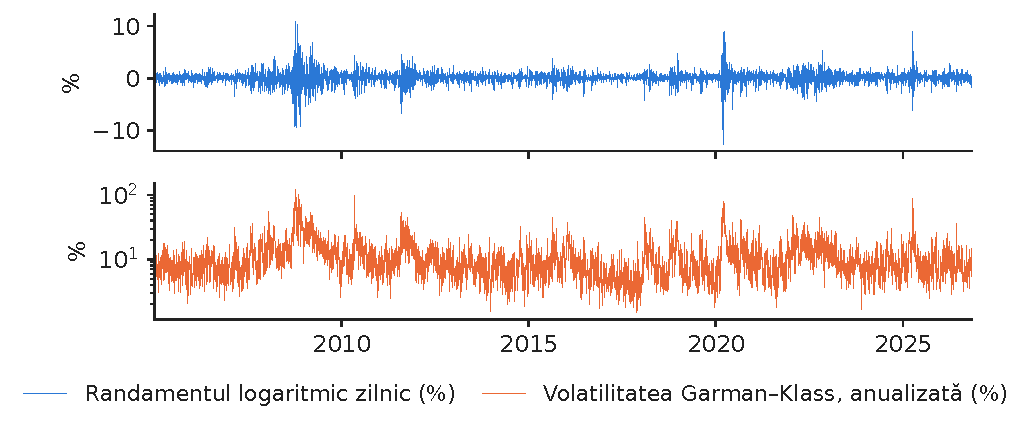
\includegraphics[width=\textwidth,height=0.420\textheight,keepaspectratio]{charts/ro/sp500_vol.pdf}\end{center}\vspace{-3mm}
\chartsource{Sursa: Yahoo Finance, cotații zilnice. Date: 4 ianuarie 2005 - 30 octombrie 2026, zile de tranzacționare.}
\vspace{0.5mm}
\begin{itemize}\setlength{\itemsep}{0pt}
  \item Estimatorul Garman--Klass (GK), din prețurile de deschidere $O_t$, maxim $H_t$, minim $L_t$ și închidere $C_t$
    \begin{itemize}\setlength{\itemsep}{0pt}
      \item Volatilitatea anualizată are mediana 8{,}77\,\% și vîrful 122\,\%, la 10 octombrie 2008.
    \end{itemize}
\end{itemize}
\par\vfill\noindent{\scriptsize\color{FooterGray}(Garman \& Klass, 1980; calcul propriu)}\hfill\qlink{NN\_L5\_sp500\_vol}{Quantlets/L5/NN_L5_sp500_vol}\par\vspace{0.5mm}
\end{frame}

\begin{frame}{Autocorelația randamentelor și a randamentelor absolute}
\small
\intuition{autocorelațiile lui $|r_t|$ rămîn pozitive luni întregi; cele ale lui $r_t$ sînt în banda de zgomot.}
\vspace{-1mm}\[ \hat\rho(k)=\frac{\sum_{t=k+1}^{T}(x_t-\bar x)(x_{t-k}-\bar x)}{\sum_{t=1}^{T}(x_t-\bar x)^2} \]\vspace{-2mm}
\begin{center}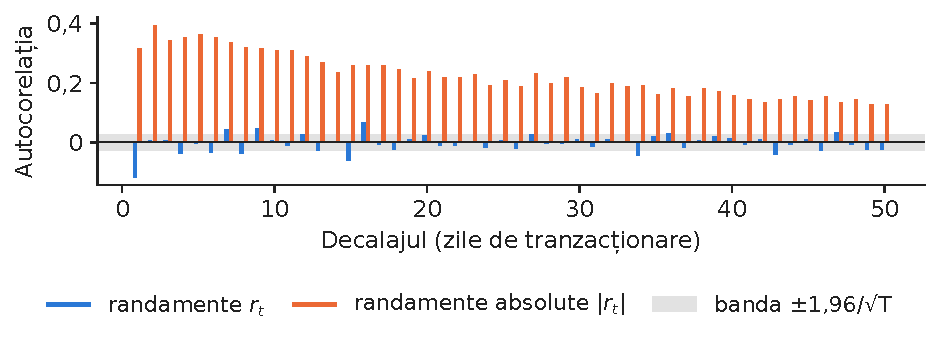
\includegraphics[width=\textwidth,height=0.272\textheight,keepaspectratio]{charts/ro/acf_abs.pdf}\end{center}\vspace{-3mm}
\chartsource{Sursa: Yahoo Finance, cotații zilnice. Date: 4 ianuarie 2005 - 30 octombrie 2026, zile de tranzacționare.}
\vspace{0.5mm}
\begin{itemize}\setlength{\itemsep}{0pt}
  \item $\hat\rho_r(1)=\ensuremath{-}0{,}119$, dar $\hat\rho_{|r|}(1)=0{,}315$ și $\hat\rho_{|r|}(50)=0{,}126$
    \begin{itemize}\setlength{\itemsep}{0pt}
      \item Banda $\pm0{,}026$
      \item Decalaje semnificative din 50: 15 pentru $r_t$, 50 pentru $|r_t|$.
    \end{itemize}
\end{itemize}
\par\vfill\manager{un model cu memorie merită încercat pentru risc (volatilitate, valoarea expusă la risc (VaR)), mult mai puțin pentru direcția prețului.}\par\vspace{0.5mm}
\par\vfill\noindent{\scriptsize\color{FooterGray}(calcul propriu)}\hfill\qlink{NN\_L5\_acf\_abs}{Quantlets/L5/NN_L5_acf_abs}\par\vspace{0.5mm}
\end{frame}

\begin{frame}{Memoria limitată a unui MLP pe fereastră fixă}
\footnotesize
\intuition{un MLP aplicat ultimelor $W$ observații are ponderi separate pentru fiecare decalaj și o limită strictă de memorie.}
\begin{columns}[T,onlytextwidth]
\begin{column}{0.53\textwidth}
\[ \hat y_{t+1}=g\big(\mW[\mathbf x_{t-W+1};\dots;\mathbf x_t]+\vb\big),\qquad \mW\in\R^{m\times Wd} \]{\footnotesize\begin{itemize}\setlength{\itemsep}{0pt}
  \item \textbf{\txtwhere}
    \begin{itemize}\setlength{\itemsep}{0pt}
      \item $\mathbf x_t\in\R^d$ intrările zilei $t$
      \item $W$ lungimea ferestrei
      \item $m$ unitățile ascunse
      \item Numărul de parametri crește liniar cu $W$
    \end{itemize}
\end{itemize}\par}
\end{column}
\begin{column}{0.44\textwidth}
\begin{itemize}\setlength{\itemsep}{2pt}
  \item \textbf{Ce ne dorim în schimb}
    \begin{itemize}\setlength{\itemsep}{0pt}
      \item O stare $\vh_t$ care rezumă trecutul
      \item Aceeași regulă de actualizare la fiecare pas (ponderi partajate în timp, ca o rețea neuronală convoluțională (CNN) în spațiu)
      \item Orice lungime a secvenței
    \end{itemize}
\end{itemize}
\end{column}
\end{columns}
\par\vfill\manager{în producție, starea se actualizează la fiecare observație nouă, fără a recalcula întregul istoric.}\par\vspace{0.5mm}
\par\vfill\noindent{\scriptsize\color{FooterGray}(Bishop \& Bishop, 2024, cap.~12)}\par\vspace{0.5mm}
\end{frame}


\section{Rețeaua recurentă și propagarea înapoi în timp}

\begin{frame}{RNN simplă: o stare, actualizată după aceeași regulă}
\footnotesize
\intuition{noua stare combină starea veche cu intrarea nouă printr-o funcție neliniară.}
\begin{columns}[T,onlytextwidth]
\begin{column}{0.53\textwidth}
\[ \vh_t=\tanh(\mW_{xh}\vx_t+\mW_{hh}\vh_{t-1}+\vb_h),\qquad \hat y_t=\mW_{hy}\vh_t+b_y \]{\footnotesize\begin{itemize}\setlength{\itemsep}{0pt}
  \item \textbf{\txtwhere}
    \begin{itemize}\setlength{\itemsep}{0pt}
      \item $\vh_t\in\R^{n_h}$ starea ascunsă, $\vh_0=\mathbf 0$
      \item $\mW_{xh}\in\R^{n_h\times d}$, $\mW_{hh}\in\R^{n_h\times n_h}$ comune pentru toți $t$
      \item Parametri $n_h(d+n_h+1)+n_h+1$, independenți de lungimea $T$
    \end{itemize}
\end{itemize}\par}
\end{column}
\begin{column}{0.44\textwidth}
\begin{itemize}\setlength{\itemsep}{2pt}
  \item Desfășurată în timp, este o rețea adîncă de adîncime $T$, cu ponderi legate.
  \item Modelul nostru de volatilitate: $d=3$ intrări (log-varianța, randamentul, randamentul absolut), $n_h=32$, fereastră de $T=22$ de zile de tranzacționare.
  \item Many-to-one: doar $\hat y_T$ (log-varianța de mîine) intră în funcția de pierdere.
\end{itemize}
\end{column}
\end{columns}
\par\vfill\manager{starea ascunsă este un analog învățat și neliniar al varianței condiționate dintr-un model GARCH.}\par\vspace{0.5mm}
\par\vfill\noindent{\scriptsize\color{FooterGray}(Rumelhart et al., 1986; Bishop \& Bishop, 2024, secț.~12.2)}\par\vspace{0.5mm}
\end{frame}

\begin{frame}{Propagarea înapoi în timp: o sumă peste drumuri}
\footnotesize
\intuition{gradientul unei ponderi comune adună contribuția ei de la fiecare pas, fiecare trecînd printr-un produs de matrice jacobiene.}
\begin{columns}[T,onlytextwidth]
\begin{column}{0.53\textwidth}
\[ \frac{\partial\loss_T}{\partial\mW_{hh}}=\sum_{t=1}^{T}\frac{\partial\loss_T}{\partial\vh_T}\Big(\prod_{s=t+1}^{T}\mathbf J_s\Big)\frac{\partial^{+}\vh_t}{\partial\mW_{hh}} \]\vspace{-2mm}\[ \mathbf J_s=\frac{\partial\vh_s}{\partial\vh_{s-1}}=\mathrm{diag}(1-\vh_s^{2})\mW_{hh} \]{\footnotesize\begin{itemize}\setlength{\itemsep}{0pt}
  \item \textbf{\txtwhere}
    \begin{itemize}\setlength{\itemsep}{0pt}
      \item $\partial^{+}$ derivata imediată, cu $\vh_{t-1}$ fixat
      \item $\mathbf J_s$ matricea jacobiană a unui pas
      \item Derivarea completă este în anexă
    \end{itemize}
\end{itemize}\par}
\end{column}
\begin{column}{0.44\textwidth}
\begin{itemize}\setlength{\itemsep}{2pt}
  \item Cost: o trecere înapoi prin toți cei $T$ pași, memorie $O(T n_h)$.
  \item BPTT trunchiată: propagare înapoi doar pe $K<T$ pași
    \begin{itemize}\setlength{\itemsep}{0pt}
      \item Mai ieftin, dar fără semnal de gradient dincolo de $K$.
    \end{itemize}
\end{itemize}
\end{column}
\end{columns}
\par\vfill\manager{produsul celor $T-t$ matrice jacobiene decide ce poate învăța rețeaua din trecutul îndepărtat.}\par\vspace{0.5mm}
\par\vfill\noindent{\scriptsize\color{FooterGray}(Werbos, 1990)}\par\vspace{0.5mm}
\end{frame}

\begin{frame}{Gradienți care dispar și gradienți care explodează}
\footnotesize
\intuition{un produs de multe matrice scade sau crește geometric cu distanța în timp.}
\begin{columns}[T,onlytextwidth]
\begin{column}{0.53\textwidth}
\[ \Big\|\prod_{s=t+1}^{T}\mathbf J_s\Big\|\le\big(\gamma\,\sigma_{\max}(\mW_{hh})\big)^{T-t},\qquad \gamma=\max|\tanh'|\le1 \]{\footnotesize\begin{itemize}\setlength{\itemsep}{0pt}
  \item \textbf{\txtwhere}
    \begin{itemize}\setlength{\itemsep}{0pt}
      \item $\sigma_{\max}$ cea mai mare valoare singulară
      \item Dacă $\gamma\sigma_{\max}<1$, marginea dispare geometric (condiție suficientă)
      \item O valoare proprie maximă peste 1 este necesară pentru explozie
    \end{itemize}
\end{itemize}\par}
\end{column}
\begin{column}{0.44\textwidth}
\begin{itemize}\setlength{\itemsep}{2pt}
  \item \textbf{Explozia}: limitarea normei gradientului
    \begin{itemize}\setlength{\itemsep}{0pt}
      \item $\mathbf g\leftarrow\mathbf g\cdot\min(1,\,c/\|\mathbf g\|)$; folosim $c=1$ (ales a priori)
    \end{itemize}
  \item \textbf{Dispariția}: schimbarea arhitecturii
    \begin{itemize}\setlength{\itemsep}{0pt}
      \item Un drum aditiv prin timp: celulele LSTM și GRU, în secțiunea următoare
    \end{itemize}
\end{itemize}
\end{column}
\end{columns}
\par\vfill\manager{în practică, o RNN simplă își amintește cîteva zeci de pași: suficient pentru volatilitatea zilnică, nu pentru tiparele săptămînale din datele orare.}\par\vspace{0.5mm}
\par\vfill\noindent{\scriptsize\color{FooterGray}(Bengio et al., 1994; Pascanu et al., 2013)}\par\vspace{0.5mm}
\end{frame}


\section{Celule cu porți: LSTM și GRU}

\begin{frame}{Celula LSTM, poartă cu poartă}
\footnotesize
\intuition{o stare separată a celulei, $\mathbf c_t$, se actualizează aditiv; trei porți decid ce se uită, ce se scrie și ce se arată.}
\begin{columns}[T,onlytextwidth]
\begin{column}{0.6\textwidth}
\[\begin{aligned} \mathbf f_t&=\sigma(\mW_f[\vh_{t-1};\vx_t]+\vb_f), & \mathbf i_t&=\sigma(\mW_i[\vh_{t-1};\vx_t]+\vb_i),\\ \mathbf o_t&=\sigma(\mW_o[\vh_{t-1};\vx_t]+\vb_o), & \tilde{\mathbf c}_t&=\tanh(\mW_c[\vh_{t-1};\vx_t]+\vb_c),\\ \mathbf c_t&=\mathbf f_t\odot\mathbf c_{t-1}+\mathbf i_t\odot\tilde{\mathbf c}_t, & \vh_t&=\mathbf o_t\odot\tanh(\mathbf c_t) \end{aligned}\]{\footnotesize\begin{itemize}\setlength{\itemsep}{0pt}
  \item \textbf{\txtwhere}
    \begin{itemize}\setlength{\itemsep}{0pt}
      \item $\sigma$ funcția logistică, cu valori în $(0,1)$
      \item $\odot$ produsul element cu element
      \item $\mathbf f,\mathbf i,\mathbf o$ porțile de uitare, intrare și ieșire
      \item Parametri $4n_h(n_h+d+1)$
    \end{itemize}
\end{itemize}\par}
\end{column}
\begin{column}{0.37\textwidth}
\begin{itemize}\setlength{\itemsep}{2pt}
  \item Poarta de uitare aproape de 1: celula își păstrează memoria
    \begin{itemize}\setlength{\itemsep}{0pt}
      \item Aproape de 0: o resetează.
    \end{itemize}
  \item Poarta de intrare: cît din candidatul $\tilde{\mathbf c}_t$ se scrie.
  \item Poarta de ieșire: cît din memorie apare în $\vh_t$.
\end{itemize}
\end{column}
\end{columns}
\par\vfill\manager{porțile sînt comutatoare învățate
    \begin{itemize}\setlength{\itemsep}{0pt}
      \item Pe datele de piață ele reacționează la șocuri (două diapozitive mai încolo).
    \end{itemize}}\par\vspace{0.5mm}
\par\vfill\noindent{\scriptsize\color{FooterGray}(Hochreiter \& Schmidhuber, 1997)}\par\vspace{0.5mm}
\end{frame}

\begin{frame}{De ce starea celulei duce gradienții departe în trecut}
\footnotesize
\intuition{de-a lungul stării celulei, jacobianul este o diagonală de porți de uitare, nu o matrice de ponderi comprimată de $\tanh'$.}
\begin{columns}[T,onlytextwidth]
\begin{column}{0.53\textwidth}
\[ \frac{\partial\mathbf c_t}{\partial\mathbf c_{t-1}}\Big|_{\text{direct}}=\mathrm{diag}(\mathbf f_t),\ \ \prod_{s=t+1}^{T}\mathrm{diag}(\mathbf f_s)\approx\mathbf I\ \text{dacă}\ \mathbf f_s\approx\mathbf 1 \]{\footnotesize\begin{itemize}\setlength{\itemsep}{0pt}
  \item \textbf{\txtwhere}
    \begin{itemize}\setlength{\itemsep}{0pt}
      \item Celelalte drumuri trec prin $\vh_{t-1}$ și prin porți
      \item Drumul direct este cel care menține gradienții pe distanțe lungi
    \end{itemize}
\end{itemize}\par}
\end{column}
\begin{column}{0.44\textwidth}
\begin{itemize}\setlength{\itemsep}{2pt}
  \item Inițializarea pozitivă a termenului liber al porții de uitare (de exemplu 1) face $\mathbf f_t\approx\sigma(1)=0{,}73$ la început: memorie implicită.
  \item În perioada de test a volatilității, media porții de uitare este 0{,}547, iar a porții de intrare 0{,}544.
  \item Actualizarea aditivă este aceeași idee ca a conexiunii reziduale din cursul 4.
\end{itemize}
\end{column}
\end{columns}
\par\vfill\manager{alegeți LSTM sau GRU atunci cînd trecutul util este lung (o săptămînă de ore) și o RNN simplă doar pentru memorii scurte.}\par\vspace{0.5mm}
\par\vfill\noindent{\scriptsize\color{FooterGray}(Hochreiter \& Schmidhuber, 1997)}\par\vspace{0.5mm}
\end{frame}

\begin{frame}{GRU: două porți și nicio stare separată}
\footnotesize
\intuition{o poartă de actualizare interpolează între starea veche și un candidat; o poartă de resetare decide cît trecut intră în candidat.}
\begin{columns}[T,onlytextwidth]
\begin{column}{0.6\textwidth}
\[\begin{aligned} \mathbf z_t&=\sigma(\mW_z[\vh_{t-1};\vx_t]+\vb_z), & \mathbf r_t&=\sigma(\mW_r[\vh_{t-1};\vx_t]+\vb_r),\\ \tilde\vh_t&=\tanh(\mW_h[\mathbf r_t\odot\vh_{t-1};\vx_t]+\vb_h), & \vh_t&=(1-\mathbf z_t)\odot\vh_{t-1}+\mathbf z_t\odot\tilde\vh_t \end{aligned}\]{\footnotesize\begin{itemize}\setlength{\itemsep}{0pt}
  \item \textbf{\txtwhere}
    \begin{itemize}\setlength{\itemsep}{0pt}
      \item $\mathbf z_t$ poarta de actualizare
      \item $\mathbf r_t$ poarta de resetare
      \item Parametri $3n_h(n_h+d+1)$, trei sferturi dintr-un LSTM cu același $n_h$
    \end{itemize}
\end{itemize}\par}
\end{column}
\begin{column}{0.37\textwidth}
\begin{itemize}\setlength{\itemsep}{2pt}
  \item Același drum aditiv: $\partial\vh_t/\partial\vh_{t-1}\supset\mathrm{diag}(1-\mathbf z_t)$.
  \item LSTM sau GRU: nu există un cîștigător general
    \begin{itemize}\setlength{\itemsep}{0pt}
      \item Comparați-le pe datele de validare, așa cum facem mai jos.
    \end{itemize}
\end{itemize}
\end{column}
\end{columns}
\par\vfill\manager{numărul mai mic de parametri face GRU puțin mai rapidă la antrenare și mai puțin pretențioasă la date.}\par\vspace{0.5mm}
\par\vfill\noindent{\scriptsize\color{FooterGray}(Cho et al., 2014)}\par\vspace{0.5mm}
\end{frame}

\begin{frame}{Memoria măsurată: rețelele privesc la ziua de ieri și la săptămîna trecută}
\small
\intuition{sensibilitatea ieșirii rețelelor de consum antrenate la fiecare dintre cele 168 de ore de intrare, mediată pe 200 de zile de test.}
\vspace{-1mm}\[ S(k)=\frac1n\sum_{i=1}^{n}\Big|\frac{\partial\hat y_{i,12}}{\partial x_{i,\,T+1-k}}\Big| \]\vspace{-2mm}
\begin{center}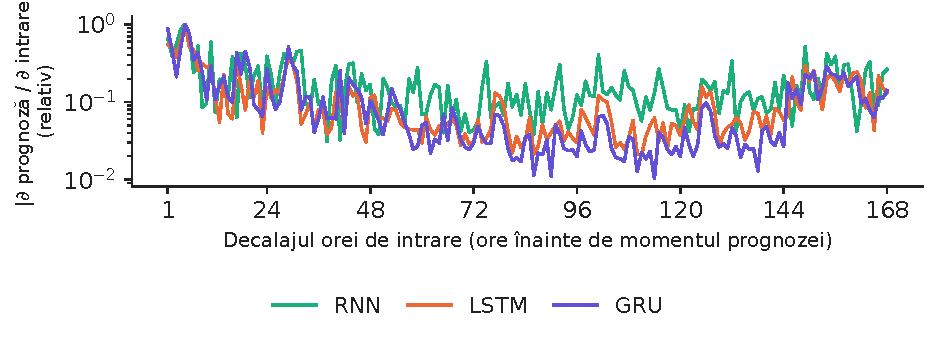
\includegraphics[width=\textwidth,height=0.319\textheight,keepaspectratio]{charts/ro/grad_lag.pdf}\end{center}\vspace{-3mm}
\chartsource{Sursa: energy-charts.info (Fraunhofer ISE), din datele burselor și ale ENTSO-E. Date: 200 de zile de test din 2024; modele cu sămînța 20261108; prognoza pentru ora 12 (timpul universal).}
\vspace{0.5mm}
\begin{itemize}\setlength{\itemsep}{0pt}
  \item Citirea a 7 profiluri zilnice în locul a 168 de ore scurtează drumul gradientului la 7 pași
    \begin{itemize}\setlength{\itemsep}{0pt}
      \item La un decalaj de o săptămînă, sensibilitatea raportată la maximul ultimei zile este RNN 0{,}261, LSTM 0{,}131, GRU 0{,}140.
    \end{itemize}
\end{itemize}
\par\vfill\noindent{\scriptsize\color{FooterGray}(calcul propriu)}\hfill\qlink{NN\_L5\_grad\_lag}{Quantlets/L5/NN_L5_grad_lag}\par\vspace{0.5mm}
\end{frame}

\begin{frame}{Porțile LSTM reacționează la stresul din piață}
\small
\intuition{activările porților LSTM-ului de volatilitate antrenat, în anii de test 2020--2026 (medii pe 5 zile).}
\begin{center}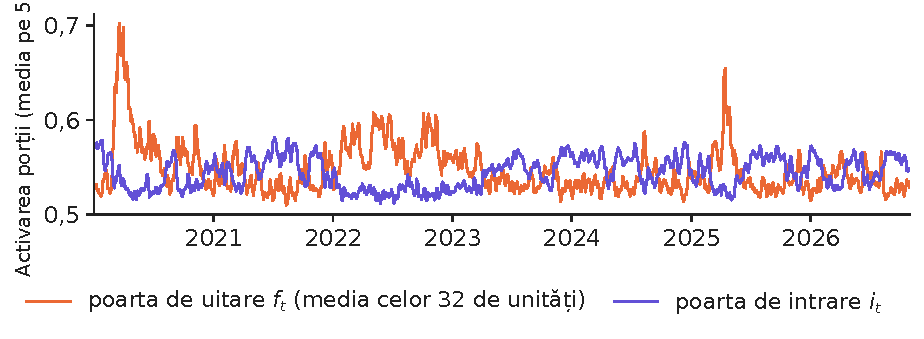
\includegraphics[width=\textwidth,height=0.362\textheight,keepaspectratio]{charts/ro/lstm_gates.pdf}\end{center}\vspace{-3mm}
\chartsource{Sursa: Yahoo Finance, cotații zilnice. Date: perioada de test 2020-2026, LSTM cu sămînța 20261108, ultimul pas al fiecărei ferestre de 22 de zile.}
\vspace{0.5mm}
\begin{itemize}\setlength{\itemsep}{0pt}
  \item Corelația cu log-varianța de azi: poarta de uitare 0{,}743, poarta de intrare \ensuremath{-}0{,}616.
\end{itemize}
\par\vfill\manager{porțile sînt un instrument de diagnostic, nu o explicație: folosiți-le pentru a vedea cînd își schimbă modelul regimul, apoi verificați pe date.}\par\vspace{0.5mm}
\par\vfill\noindent{\scriptsize\color{FooterGray}(calcul propriu)}\hfill\qlink{NN\_L5\_lstm\_gates}{Quantlets/L5/NN_L5_lstm_gates}\par\vspace{0.5mm}
\end{frame}

\begin{frame}{Arhitecturi pentru secvențe și scurgerea de informație din viitor}
\footnotesize
\begin{columns}[T,onlytextwidth]
\begin{column}{0.49\textwidth}
\begin{itemize}\setlength{\itemsep}{4pt}
  \item \textbf{Many-to-one}
    \begin{itemize}\setlength{\itemsep}{0pt}
      \item O fereastră la intrare, o valoare la ieșire: volatilitatea de mîine
    \end{itemize}
  \item \textbf{Many-to-many (ieșire vectorială)}
    \begin{itemize}\setlength{\itemsep}{0pt}
      \item O săptămînă de profiluri zilnice la intrare, cele 24 de ore de mîine la ieșire: modelul nostru de consum
    \end{itemize}
  \item \textbf{Codificator--decodificator}
    \begin{itemize}\setlength{\itemsep}{0pt}
      \item O rețea citește, alta scrie o secvență pas cu pas
    \end{itemize}
\end{itemize}
\end{column}
\begin{column}{0.48\textwidth}
\begin{itemize}\setlength{\itemsep}{4pt}
  \item \textbf{Straturi suprapuse}
    \begin{itemize}\setlength{\itemsep}{0pt}
      \item Stările stratului 1 sînt intrările stratului 2
    \end{itemize}
  \item \textbf{Bidirecțional (BiLSTM)}
    \begin{itemize}\setlength{\itemsep}{0pt}
      \item Citește fereastra înainte și înapoi
      \item Potrivit pentru clasificarea unui text sau a unei secvențe încheiate
      \item O scurgere de informație în prognoză dacă trecerea înapoi vede viitorul
    \end{itemize}
\end{itemize}
\end{column}
\end{columns}
\par\vfill\manager{în prognoză, fiecare intrare trebuie să fie cunoscută în momentul prognozei: verificați acest lucru înaintea oricărei alegeri de arhitectură.}\par\vspace{0.5mm}
\par\vfill\noindent{\scriptsize\color{FooterGray}(Bishop \& Bishop, 2024, cap.~12)}\par\vspace{0.5mm}
\end{frame}


\section{Un protocol pentru serii de timp financiare}

\begin{frame}{Ferestre, scalare și împărțiri fără scurgeri de informație}
\footnotesize
\intuition{fiecare număr pe care îl vede modelul trebuie să poată fi calculat în momentul prognozei $t$.}
\begin{columns}[T,onlytextwidth]
\begin{column}{0.53\textwidth}
\[ \mathcal D=\{(\mathbf x_{t-W+1:t},\,y_{t+1})\},\qquad \tilde x=\frac{x-\bar x_{\mathrm{train}}}{s_{\mathrm{train}}} \]{\footnotesize\begin{itemize}\setlength{\itemsep}{0pt}
  \item \textbf{\txtwhere}
    \begin{itemize}\setlength{\itemsep}{0pt}
      \item $W$ fereastra
      \item $\bar x_{\mathrm{train}},s_{\mathrm{train}}$ media și abaterea standard calculate numai pe anii de antrenare
    \end{itemize}
\end{itemize}\par}
\end{column}
\begin{column}{0.44\textwidth}
\begin{itemize}\setlength{\itemsep}{2pt}
  \item S\&P 500: 3\,020 de zile de antrenare, 754 de validare și 1\,717 de test, în această ordine.
  \item Oprirea timpurie: ne oprim cînd pierderea de validare nu s-a îmbunătățit timp de 6 epoci
    \begin{itemize}\setlength{\itemsep}{0pt}
      \item Păstrăm cele mai bune ponderi.
    \end{itemize}
  \item Semințe: cîte 5 pentru fiecare rețea (volatilitate, randamente), 3 pentru consum
    \begin{itemize}\setlength{\itemsep}{0pt}
      \item Raportăm dispersia și prognoza medie.
    \end{itemize}
\end{itemize}
\end{column}
\end{columns}
\par\vfill\manager{o amestecare aleatoare a zilelor înainte de împărțire pune anul 2020 în setul de antrenare și face orice model să pară bun pe 2020.}\par\vspace{0.5mm}
\par\vfill\noindent{\scriptsize\color{FooterGray}(calcul propriu)}\hfill\tryit{\S2}\par\vspace{0.5mm}
\end{frame}

\begin{frame}{Întîi modelele de referință: naiv, HAR și GARCH}
\footnotesize
\intuition{o rețea trebuie să depășească modele pe care econometria le-a rafinat de decenii.}
\begin{columns}[T,onlytextwidth]
\begin{column}{0.53\textwidth}
\[\begin{aligned} \text{HAR: } y_{t+1}&=\beta_0+\beta_d y_t+\beta_w\bar y_{t-4:t}+\beta_m\bar y_{t-21:t}\\ \text{GARCH(1,1): } \sigma^2_{t+1}&=\omega+\alpha\,\varepsilon_t^2+\beta\,\sigma^2_t,\quad \varepsilon_t=r_t-\mu \end{aligned}\]{\footnotesize\begin{itemize}\setlength{\itemsep}{0pt}
  \item \textbf{\txtwhere}
    \begin{itemize}\setlength{\itemsep}{0pt}
      \item $y_t=\ln\hat\sigma^2_{\mathrm{GK},t}$
      \item $\bar y$ medii pe o săptămînă și pe o lună
      \item GARCH cu erori Student-$t$, raportat la $y$ printr-o regresie liniară pe anii de antrenare
      \item Naiv: $\hat y_{t+1}=y_t$
    \end{itemize}
\end{itemize}\par}
\end{column}
\begin{column}{0.44\textwidth}
\begin{itemize}\setlength{\itemsep}{2pt}
  \item Estimările modelului HAR: $\hat\beta_d=0{,}192$, $\hat\beta_w=0{,}439$, $\hat\beta_m=0{,}293$.
  \item GARCH: $\hat\alpha=0{,}117$, $\hat\beta=0{,}873$, persistență 0{,}990, $\hat\nu=5{,}78$.
\end{itemize}
\end{column}
\end{columns}
\par\vfill\manager{HAR este un model liniar cu trei medii
    \begin{itemize}\setlength{\itemsep}{0pt}
      \item Dacă un LSTM nu îl poate depăși, LSTM-ul nu merită întreținut.
    \end{itemize}}\par\vspace{0.5mm}
\par\vfill\noindent{\scriptsize\color{FooterGray}(Corsi, 2009; Bollerslev, 1986)}\par\vspace{0.5mm}
\end{frame}

\begin{frame}{Este o prognoză într-adevăr mai bună? Testul Diebold--Mariano}
\footnotesize
\intuition{comparăm zi de zi pierderile a două prognoze și testăm dacă diferența lor medie este zero.}
\begin{columns}[T,onlytextwidth]
\begin{column}{0.53\textwidth}
\[ d_t=L(e_{1,t})-L(e_{2,t}),\qquad \mathrm{DM}=\frac{\bar d}{\sqrt{\hat\sigma^2_{\mathrm{NW}}/n}}\;\overset{H_0}{\sim}\;\mathcal N(0,1) \]{\footnotesize\begin{itemize}\setlength{\itemsep}{0pt}
  \item \textbf{\txtwhere}
    \begin{itemize}\setlength{\itemsep}{0pt}
      \item $L$ eroarea pătratică (volatilitate) sau eroarea absolută (consum)
      \item $\hat\sigma^2_{\mathrm{NW}}$ varianța de termen lung Newey--West a lui $d_t$
      \item $\mathrm{DM}<0$: modelul 1 este mai bun
    \end{itemize}
\end{itemize}\par}
\end{column}
\begin{column}{0.44\textwidth}
\begin{itemize}\setlength{\itemsep}{2pt}
  \item Testul Diebold--Mariano (DM) ține seama de autocorelația diferențelor de pierdere, pe care erorile de prognoză o au întotdeauna.
  \item Semințele măsoară zgomotul antrenării
    \begin{itemize}\setlength{\itemsep}{0pt}
      \item DM măsoară zgomotul de eșantionare al perioadei de test.
    \end{itemize}
\end{itemize}
\end{column}
\end{columns}
\par\vfill\manager{declarați un model mai bun doar cu valoarea $p$ a testului DM și precizați perioada.}\par\vspace{0.5mm}
\par\vfill\noindent{\scriptsize\color{FooterGray}(Diebold \& Mariano, 1995)}\par\vspace{0.5mm}
\end{frame}


\section{Studiul de caz A: volatilitatea S\&P 500}

\begin{frame}{În criza din 2020, LSTM s-a adaptat mai repede decît HAR}
\small
\intuition{prognoze pentru ziua următoare ale volatilității anualizate, în primul an de test.}
\vspace{-1mm}\[ \hat\sigma_{t+1}^{\mathrm{ann}}=100\sqrt{252\,\exp(\hat y_{t+1})} \]\vspace{-2mm}
\begin{center}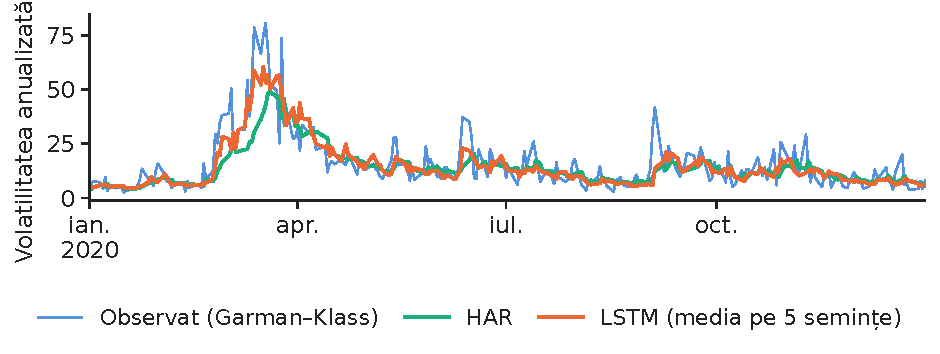
\includegraphics[width=\textwidth,height=0.420\textheight,keepaspectratio]{charts/ro/vol_forecast.pdf}\end{center}\vspace{-3mm}
\chartsource{Sursa: Yahoo Finance, cotații zilnice. Date: anul de test 2020 (prognoze pentru ziua următoare), zile de tranzacționare.}
\vspace{0.5mm}
\begin{itemize}\setlength{\itemsep}{0pt}
  \item Fereastra crizei (20 februarie -- 30 aprilie 2020), eroarea pătratică medie (MSE) a lui $\hat y$: naiv 0{,}705, GARCH 1{,}032, HAR 1{,}014, LSTM 0{,}521.
\end{itemize}
\par\vfill\noindent{\scriptsize\color{FooterGray}(calcul propriu)}\hfill\qlink{NN\_L5\_vol\_forecast}{Quantlets/L5/NN_L5_vol_forecast}\par\vspace{0.5mm}
\end{frame}

\begin{frame}{Rețelele recurente depășesc HAR și GARCH pe volatilitate}
\small
\intuition{MSE pe test a log-varianței, în perioada 2020--2026; punctele sînt semințe individuale.}
\begin{center}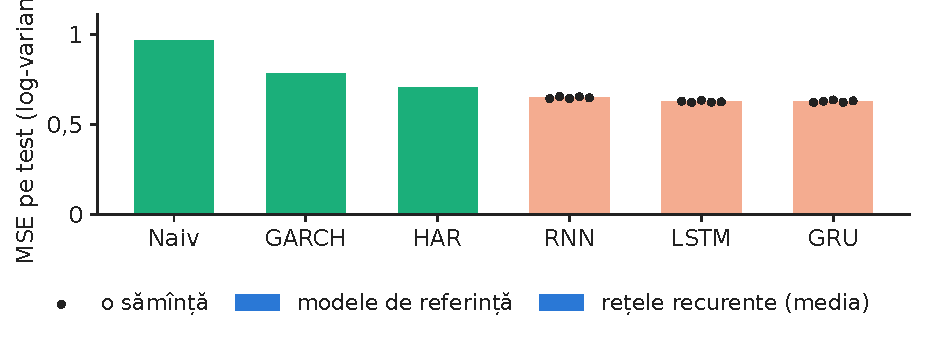
\includegraphics[width=\textwidth,height=0.420\textheight,keepaspectratio]{charts/ro/vol_mse.pdf}\end{center}\vspace{-3mm}
\chartsource{Sursa: Yahoo Finance, cotații zilnice. Date: test 2 ianuarie 2020 - 31 octombrie 2026; 5 semințe pentru fiecare rețea.}
\vspace{0.5mm}
\begin{itemize}\setlength{\itemsep}{0pt}
  \item MSE: naiv 0{,}966, GARCH 0{,}786, HAR 0{,}706
    \begin{itemize}\setlength{\itemsep}{0pt}
      \item RNN 0{,}649, LSTM 0{,}628, GRU 0{,}629 (medii pe semințe).
    \end{itemize}
\end{itemize}
\par\vfill\noindent{\scriptsize\color{FooterGray}(calcul propriu)}\hfill\qlink{NN\_L5\_vol\_mse}{Quantlets/L5/NN_L5_vol_mse}\par\vspace{0.5mm}
\end{frame}

\begin{frame}{Rezultatele pentru volatilitate, cu teste}
\footnotesize
\begin{columns}[T,onlytextwidth]
\begin{column}{0.5\textwidth}
{\footnotesize\renewcommand{\arraystretch}{1.05}\setlength{\tabcolsep}{4pt}
\begin{tabular}{@{}lrrr@{}}\toprule
Modelul & MSE & $R^2$ & Semințe \\ \midrule
Naiv & 0{,}966 & 0{,}259 & -- \\
GARCH(1,1)-$t$ & 0{,}786 & 0{,}397 & -- \\
HAR & 0{,}706 & 0{,}458 & -- \\
RNN (prognoza medie) & 0{,}643 & 0{,}507 & 5 \\
LSTM (prognoza medie) & 0{,}625 & 0{,}521 & 5 \\
GRU (prognoza medie) & 0{,}624 & 0{,}521 & 5 \\
\bottomrule\end{tabular}}
\par\vspace{0.5mm}{\scriptsize \begin{itemize}\setlength{\itemsep}{0pt}
  \item $R^2=1-\mathrm{MSE}/\widehat{\Var}(y)$ pe cele 1\,717 de zile de test.
\end{itemize}}
\end{column}
\begin{column}{0.47\textwidth}
\begin{itemize}\setlength{\itemsep}{4pt}
  \item LSTM față de HAR: variația MSE \ensuremath{-}11{,}6\,\%
    \begin{itemize}\setlength{\itemsep}{0pt}
      \item DM $=\ensuremath{-}5{,}52$, $p<0{,}001$.
    \end{itemize}
  \item LSTM față de GARCH: DM $=\ensuremath{-}6{,}80$, $p<0{,}001$.
  \item LSTM față de modelul naiv: variația MSE \ensuremath{-}35{,}3\,\%.
  \item Cea mai bună rețea după prognoza medie: GRU
    \begin{itemize}\setlength{\itemsep}{0pt}
      \item Dispersia LSTM pe semințe: între 0{,}623 și 0{,}635.
    \end{itemize}
\end{itemize}
\end{column}
\end{columns}
\par\vfill\manager{cîștigul este semnificativ pe această perioadă de test
    \begin{itemize}\setlength{\itemsep}{0pt}
      \item Înainte de a înlocui HAR într-un model VaR, verificați-l pe altă piață și pe subperioade și păstrați HAR ca soluție de rezervă.
    \end{itemize}}\par\vspace{0.5mm}
\par\vfill\noindent{\scriptsize\color{FooterGray}(calcul propriu)}\par\vspace{0.5mm}
\end{frame}


\section{Studiul de caz B: poate o rețea prognoza randamentele?}

\begin{frame}{În afara eșantionului, prognozele randamentelor nu explică aproape nimic}
\small
\intuition{randamentele de a doua zi ale S\&P 500 și ale Banca Transilvania (TLV), din ultimele 22 de randamente.}
\vspace{-1mm}\[ R^2_{\mathrm{OOS}}=1-\frac{\sum_{t\in\mathrm{test}}(r_{t+1}-\hat r_{t+1})^2}{\sum_{t\in\mathrm{test}}r_{t+1}^2} \]\vspace{-2mm}
\begin{center}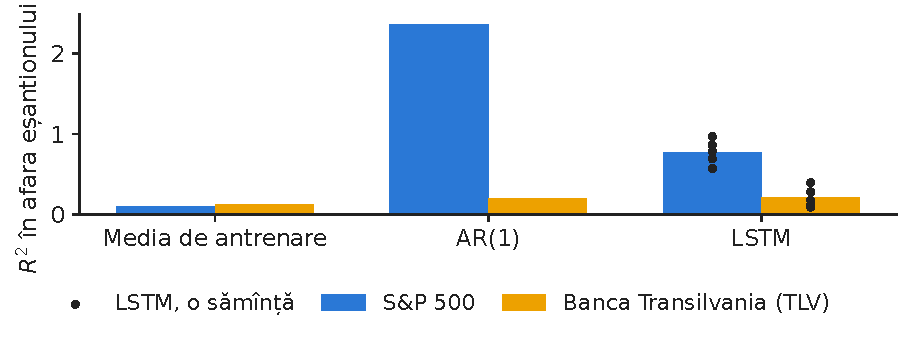
\includegraphics[width=\textwidth,height=0.383\textheight,keepaspectratio]{charts/ro/returns_r2.pdf}\end{center}\vspace{-3mm}
\chartsource{Sursa: Yahoo Finance; EODHD. Date: test 2020 - octombrie 2026; S\&P 500 (Yahoo Finance) și TLV (EODHD, Bursa de Valori București).}
\vspace{0.5mm}
\begin{itemize}\setlength{\itemsep}{0pt}
  \item S\&P 500: AR(1) 2{,}366\,\%, LSTM 0{,}776\,\% (semințe între 0{,}572 și 0{,}969)
    \begin{itemize}\setlength{\itemsep}{0pt}
      \item TLV: AR(1) 0{,}201\,\%, LSTM 0{,}213\,\%.
    \end{itemize}
\end{itemize}
\par\vfill\noindent{\scriptsize\color{FooterGray}(calcul propriu)}\hfill\qlink{NN\_L5\_returns\_r2}{Quantlets/L5/NN_L5_returns_r2}\par\vspace{0.5mm}
\end{frame}

\begin{frame}{Predictibilitatea redusă a randamentelor}
\footnotesize
\intuition{pe o piață lichidă, partea previzibilă a randamentelor este infimă față de zgomotul lor.}
\begin{columns}[T,onlytextwidth]
\begin{column}{0.53\textwidth}
\[ r_{t+1}=\mu_t+\varepsilon_{t+1},\qquad \frac{\Var(\mu_t)}{\Var(r_{t+1})}\approx0 \]{\footnotesize\begin{itemize}\setlength{\itemsep}{0pt}
  \item \textbf{\txtwhere}
    \begin{itemize}\setlength{\itemsep}{0pt}
      \item $\mu_t$ media condiționată pe care o poate învăța un model
      \item $\varepsilon_{t+1}$ știrile care apar după $t$
    \end{itemize}
\end{itemize}\par}
\end{column}
\begin{column}{0.44\textwidth}
\begin{itemize}\setlength{\itemsep}{2pt}
  \item Acuratețea semnului pentru LSTM pe testul S\&P 500: 52{,}1\,\%, față de 54{,}0\,\% zile de creștere (prognoza ``mereu în sus'').
  \item Panta AR(1) estimată pe anii de antrenare: \ensuremath{-}0{,}102 (S\&P 500), 0{,}015 (TLV).
  \item Modelele flexibile învață zgomotul în antrenare
    \begin{itemize}\setlength{\itemsep}{0pt}
      \item Oprirea timpurie limitează paguba, dar nu poate crea un semnal.
    \end{itemize}
\end{itemize}
\end{column}
\end{columns}
\par\vfill\manager{testul retrospectiv al unui furnizor de ``predicții de randamente bazate pe inteligență artificială (AI)'' trebuie să treacă acest test pe date nevăzute, după costuri.}\par\vspace{0.5mm}
\par\vfill\noindent{\scriptsize\color{FooterGray}(calcul propriu)}\par\vspace{0.5mm}
\end{frame}


\section{Studiul de caz C: consumul de energie electrică din România}

\begin{frame}{Consumul are cicluri zilnice, săptămînale și anuale}
\small
\intuition{o secvență cu memorie lungă și regulată: un candidat natural pentru rețelele recurente.}
\begin{center}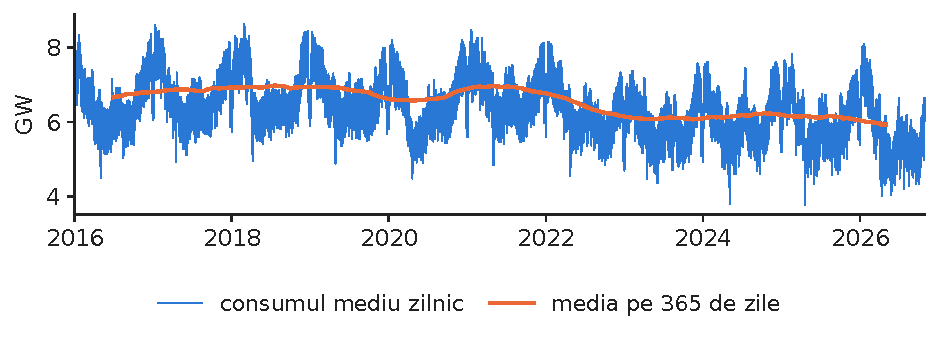
\includegraphics[width=\textwidth,height=0.420\textheight,keepaspectratio]{charts/ro/load_series.pdf}\end{center}\vspace{-3mm}
\chartsource{Sursa: energy-charts.info (Fraunhofer ISE), din datele burselor și ale ENTSO-E. Date: 1 ianuarie 2016 - 31 octombrie 2026, orar, MW medii pe zi.}
\vspace{0.5mm}
\begin{itemize}\setlength{\itemsep}{0pt}
  \item Consum orar de la 1 ianuarie 2016 la 31 octombrie 2026, în medie 6\,510 megawatt (MW)
    \begin{itemize}\setlength{\itemsep}{0pt}
      \item Cele 129 de ore lipsă rămîn lipsă (zilele respective sînt omise).
    \end{itemize}
\end{itemize}
\par\vfill\noindent{\scriptsize\color{FooterGray}(calcul propriu)}\hfill\qlink{NN\_L5\_load\_series}{Quantlets/L5/NN_L5_load_series}\par\vspace{0.5mm}
\end{frame}

\begin{frame}{Sarcina pentru ziua următoare și modelele ei de referință}
\scriptsize
\intuition{la sfîrșitul zilei $d$, prognozăm cele 24 de valori orare ale consumului din ziua $d+1$, pe baza ultimei săptămîni de ore.}
\begin{columns}[T,onlytextwidth]
\begin{column}{0.64\textwidth}
\[ \hat{\mathbf y}_{d+1}=\mathbf y_{d-6}+\mW_{o}[\vh_{7};\mathbf s_{d+1}]+\vb_o\in\R^{24} \]\vspace{-2mm}\[ \text{ARX: } \hat{\mathbf y}_{d+1}=\mathbf y_{d-6}+\mathbf B\,\mathbf x_{d,1:168}+\mathbf\Gamma\mathbf s_{d+1} \]{\footnotesize\begin{itemize}\setlength{\itemsep}{0pt}
  \item \textbf{\txtwhere}
    \begin{itemize}\setlength{\itemsep}{0pt}
      \item $\mathbf y_{d-6}$ prognoza naivă sezonieră (modelele învață corecția ei)
      \item $\vh_{7}$ ultima stare după cele 7 zile anterioare, cîte un pas pe zi (24 de valori orare + ziua săptămînii)
      \item $\mathbf s_{d+1}$ ziua săptămînii și sezonul zilei $d+1$
      \item ARX prin regresie ridge (penalizarea 1, aleasă pe anul de validare)
    \end{itemize}
\end{itemize}\par}
\end{column}
\begin{column}{0.33\textwidth}
\begin{itemize}\setlength{\itemsep}{2pt}
  \item 2\,186 de zile de antrenare, 365 de validare, 1035 de test
    \begin{itemize}\setlength{\itemsep}{0pt}
      \item 3 semințe pentru fiecare rețea.
    \end{itemize}
\end{itemize}
\end{column}
\end{columns}
\par\vfill\manager{un furnizor transmite cele 24 de volume orare înainte de prînz
    \begin{itemize}\setlength{\itemsep}{0pt}
      \item Fiecare MW de eroare se cumpără sau se vinde la prețul de dezechilibru.
    \end{itemize}}\par\vspace{0.5mm}
\par\vfill\noindent{\scriptsize\color{FooterGray}(calcul propriu)}\hfill\tryit{\S5}\par\vspace{0.5mm}
\end{frame}

\begin{frame}{Două săptămîni de test din iarnă: prognozele față de consumul observat}
\small
\intuition{consumul orar în două săptămîni de test din iarnă, observat față de două prognoze.}
\begin{center}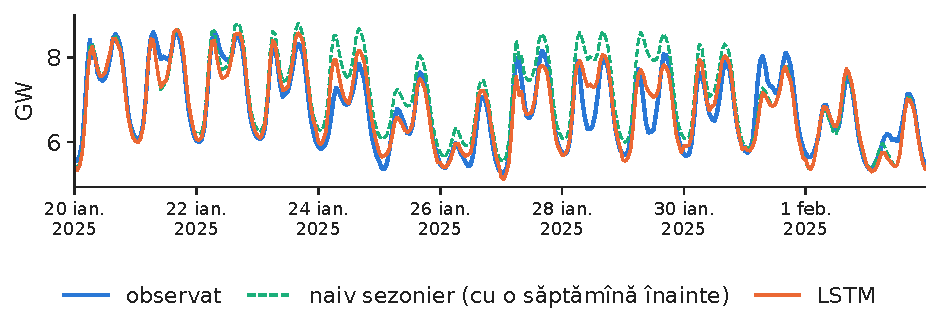
\includegraphics[width=\textwidth,height=0.450\textheight,keepaspectratio]{charts/ro/load_fortnight.pdf}\end{center}\vspace{-3mm}
\chartsource{Sursa: energy-charts.info (Fraunhofer ISE), din datele burselor și ale ENTSO-E. Date: 14 zile de test, 20 ianuarie 2025 - 2 februarie 2025.}
\vspace{0.5mm}
\begin{itemize}\setlength{\itemsep}{0pt}
  \item Prognoza naivă sezonieră copiază săptămîna trecută, inclusiv nivelul și sărbătorile ei
    \begin{itemize}\setlength{\itemsep}{0pt}
      \item Rețelele învață doar o corecție a acesteia.
    \end{itemize}
\end{itemize}
\par\vfill\noindent{\scriptsize\color{FooterGray}(calcul propriu)}\hfill\qlink{NN\_L5\_load\_fortnight}{Quantlets/L5/NN_L5_load_fortnight}\par\vspace{0.5mm}
\end{frame}

\begin{frame}{Pe consum, modelul liniar ARX depășește rețelele recurente}
\small
\intuition{stînga: eroarea procentuală absolută medie (MAPE) pe toate orele de test; dreapta: eroarea absolută medie (MAE) pe ore ale zilei.}
\vspace{-1mm}\[ \mathrm{MAPE}=\frac{100}{24n}\sum_{d}\sum_{h=1}^{24}\frac{|y_{d,h}-\hat y_{d,h}|}{y_{d,h}} \]\vspace{-2mm}
\begin{center}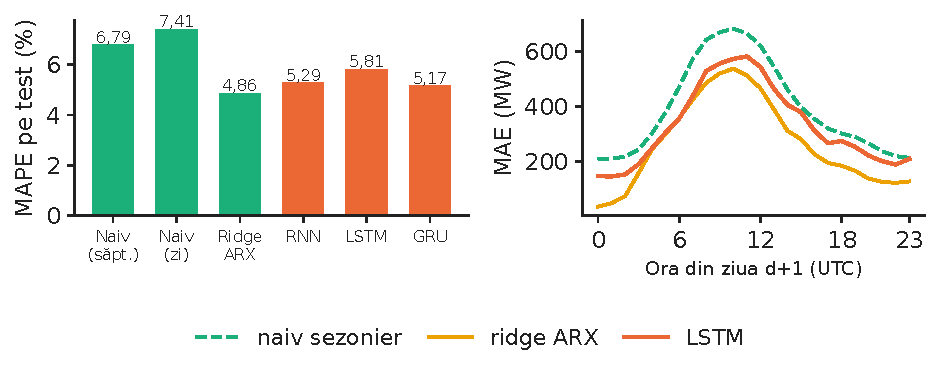
\includegraphics[width=\textwidth,height=0.381\textheight,keepaspectratio]{charts/ro/load_errors.pdf}\end{center}\vspace{-3mm}
\chartsource{Sursa: energy-charts.info (Fraunhofer ISE), din datele burselor și ale ENTSO-E. Date: 1 ianuarie 2024 - 31 octombrie 2026 (zile de test).}
\vspace{0.5mm}
\begin{itemize}\setlength{\itemsep}{0pt}
  \item MAPE (\%): naiv sezonier 6{,}79, naiv 7{,}41, ridge ARX 4{,}86, RNN 5{,}29, LSTM 5{,}81, GRU 5{,}17.
\end{itemize}
\par\vfill\noindent{\scriptsize\color{FooterGray}(calcul propriu)}\hfill\qlink{NN\_L5\_load\_errors}{Quantlets/L5/NN_L5_load_errors}\par\vspace{0.5mm}
\end{frame}

\begin{frame}{Ferestrele mai lungi ajută LSTM, pînă la o săptămînă}
\small
\intuition{eroarea LSTM pe test în funcție de fereastra de intrare, cu același protocol în rest.}
\begin{center}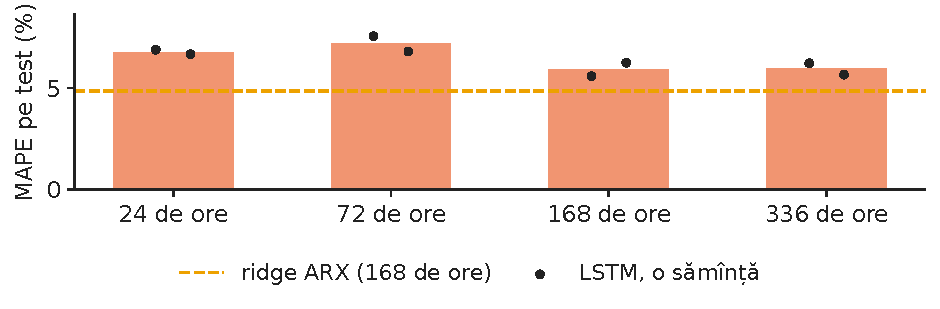
\includegraphics[width=\textwidth,height=0.420\textheight,keepaspectratio]{charts/ro/load_window.pdf}\end{center}\vspace{-3mm}
\chartsource{Sursa: energy-charts.info (Fraunhofer ISE), din datele burselor și ale ENTSO-E. Date: zile de test 2024-2026; LSTM cu 2 semințe pentru fiecare fereastră.}
\vspace{0.5mm}
\begin{itemize}\setlength{\itemsep}{0pt}
  \item MAPE (\%): 24 de ore 6{,}77, 72 de ore 7{,}17, 168 de ore 5{,}91, 336 de ore 5{,}93.
\end{itemize}
\par\vfill\noindent{\scriptsize\color{FooterGray}(calcul propriu)}\hfill\qlink{NN\_L5\_load\_window}{Quantlets/L5/NN_L5_load_window}\par\vspace{0.5mm}
\end{frame}

\begin{frame}{Cît valorează o prognoză mai bună a consumului}
\footnotesize
\begin{itemize}\setlength{\itemsep}{4pt}
  \item \textbf{Semnificația}
    \begin{itemize}\setlength{\itemsep}{0pt}
      \item Cea mai bună rețea după prognoza medie: GRU, MAPE cu \ensuremath{+}6{,}4\,\% față de ridge ARX: cu 2\,186 de zile de antrenare, modelul liniar cîștigă
      \item DM pe MAE zilnic, LSTM față de ridge ARX: 9{,}80, $p<0{,}001$
    \end{itemize}
  \item \textbf{În megawați}
    \begin{itemize}\setlength{\itemsep}{0pt}
      \item Eroarea absolută medie pe oră: naiv sezonier 396 MW, ridge ARX 269 MW, LSTM 331 MW
      \item LSTM în locul prognozei naive sezoniere: cu aproximativ 1\,560 megawați-oră (MWh) mai puțină eroare absolută pe zi, la scară națională
    \end{itemize}
  \item \textbf{Costul}
    \begin{itemize}\setlength{\itemsep}{0pt}
      \item Antrenarea tuturor modelelor de consum și studiul ferestrei: 67 de secunde pe procesorul central al unui laptop
    \end{itemize}
\end{itemize}
\par\vfill\manager{înmulțiți MWh economisiți cu diferența de preț de dezechilibru și comparați cu costul modelului: aici ridge ARX economisește cel mai mult cu cel mai mic cost
    \begin{itemize}\setlength{\itemsep}{0pt}
      \item Variabilele meteo ar aduce un plus (cursul 13).
    \end{itemize}}\par\vspace{0.5mm}
\par\vfill\noindent{\scriptsize\color{FooterGray}(calcul propriu)}\par\vspace{0.5mm}
\end{frame}

\section*{Recapitulare}

\begin{frame}{Test 1: parametrii}
\small
\begin{itemize}
  \item Cîți parametri are un strat LSTM cu $d=3$ intrări și $n_h=32$ de unități?
\end{itemize}
\vspace{2mm}
\begin{exampleblock}{R\u{a}spuns}
\begin{itemize}
  \item $4n_h(n_h+d+1)=4\cdot32\cdot36=4608$ (PyTorch păstrează doi vectori de termeni liberi, deci raportează $4608+128=4736$).
\end{itemize}
\end{exampleblock}
\end{frame}

\begin{frame}{Test 2: gradienții}
\small
\begin{itemize}
  \item De ce are o RNN simplă dificultăți cu tiparul săptămînal al consumului orar?
\end{itemize}
\vspace{2mm}
\begin{exampleblock}{R\u{a}spuns}
\begin{itemize}
  \item Pe 168 de pași orari, gradientul este un produs de 168 de matrice jacobiene și dispare
    \begin{itemize}\setlength{\itemsep}{0pt}
      \item Citirea a 7 profiluri zilnice scurtează drumul la 7 pași, iar așa sînt construite modelele noastre de consum.
    \end{itemize}
\end{itemize}
\end{exampleblock}
\end{frame}

\begin{frame}{Test 3: afirmația unui furnizor}
\small
\begin{itemize}
  \item Un furnizor prezintă un LSTM cu acuratețe de 60\,\% a semnului randamentelor S\&P 500, antrenat pe zile amestecate
    \begin{itemize}\setlength{\itemsep}{0pt}
      \item Ce întrebați?
    \end{itemize}
\end{itemize}
\vspace{2mm}
\begin{exampleblock}{R\u{a}spuns}
\begin{itemize}
  \item Un test în ordine cronologică, pe ani nevăzuți, față de prognoza ``mereu în sus'' (54{,}0\,\%) și după costuri
    \begin{itemize}\setlength{\itemsep}{0pt}
      \item LSTM-ul nostru, evaluat corect, atinge 52{,}1\,\%.
    \end{itemize}
\end{itemize}
\end{exampleblock}
\end{frame}

\begin{frame}{Test 4: HAR sau LSTM}
\small
\begin{itemize}
  \item LSTM schimbă MSE a volatilității cu \ensuremath{-}11{,}6\,\% față de HAR, cu DM $=\ensuremath{-}5{,}52$
    \begin{itemize}\setlength{\itemsep}{0pt}
      \item Înlocuiește HAR în sistemul VaR?
    \end{itemize}
\end{itemize}
\vspace{2mm}
\begin{exampleblock}{R\u{a}spuns}
\begin{itemize}
  \item Cîștigul este semnificativ aici, deci LSTM este un candidat serios
    \begin{itemize}\setlength{\itemsep}{0pt}
      \item Schimbați modelul doar după ce cîștigul se confirmă pe altă piață și pe subperioade, cu monitorizare și cu HAR ca soluție de rezervă.
    \end{itemize}
\end{itemize}
\end{exampleblock}
\end{frame}

\begin{frame}{Test 5: bidirecțional}
\small
\begin{itemize}
  \item Puteți folosi un LSTM bidirecțional pentru a prognoza consumul de mîine dintr-o fereastră care se termină azi?
\end{itemize}
\vspace{2mm}
\begin{exampleblock}{R\u{a}spuns}
\begin{itemize}
  \item Da, dacă fereastra se termină în momentul prognozei: trecerea înapoi vede atunci doar trecutul
    \begin{itemize}\setlength{\itemsep}{0pt}
      \item Apare o scurgere doar dacă fereastra conține ore de după acel moment.
    \end{itemize}
\end{itemize}
\end{exampleblock}
\end{frame}

\begin{frame}{Recapitulare}
\small
\vspace{-2mm}\begin{multicols}{2}\scriptsize\tableofcontents\end{multicols}
\begin{itemize}\setlength{\itemsep}{1pt}
  \item O RNN partajează ponderile în timp
    \begin{itemize}\setlength{\itemsep}{0pt}
      \item BPTT înmulțește matrice jacobiene, deci gradienții dispar sau explodează
      \item LSTM și GRU adaugă un drum aditiv al memoriei.
    \end{itemize}
  \item Pe date reale: rețelele depășesc HAR pe volatilitate, prognozele randamentelor nu explică aproape nimic, iar un ARX liniar cîștigă pe consumul orar
    \begin{itemize}\setlength{\itemsep}{0pt}
      \item Urmează textul (cursul 6).
    \end{itemize}
\end{itemize}
\end{frame}

\begin{frame}{Cercetări ale grupului nostru: secvențe și risc}
\footnotesize
\begin{itemize}\setlength{\itemsep}{3pt}
  \item \textbf{Pot gestiona riscul modelele fundaționale?} (Jheng, Tak, Găman, Mazurencu-Marinescu-Pele \& Pele, 2026, Economic Computation and Economic Cybernetics Studies and Research)
    \begin{itemize}\setlength{\itemsep}{0pt}
      \item Modele preantrenate pentru serii de timp, folosite fără reantrenare pentru prognoza VaR și a pierderii medii peste VaR (ES) pe piețele din Europa Centrală și de Est (CEE)
      \item O calibrare conformală face fiabile prognozele de coadă; succesorii transformer ai LSTM sînt prezentați în cursurile 7 și 13
    \end{itemize}
  \item \textbf{Avertizarea timpurie pentru criptoactivele ``zombie''} (Będowska-Sójka, Wójcik \& Pele, 2026, North American Journal of Economics and Finance)
    \begin{itemize}\setlength{\itemsep}{0pt}
      \item Un sistem de avertizare timpurie bazat pe învățare automată pentru criptoactivele care își pierd activitatea de piață
    \end{itemize}
  \item \textbf{BitMood} (Conda, Găman, Bâg, Mazurencu-Marinescu-Pele, Pele \& Härdle, 2026, Digital Finance)
    \begin{itemize}\setlength{\itemsep}{0pt}
      \item Sentimentul de pe Facebook și volumul Bitcoin: regresia liniară și un LSTM bidirecțional au performanțe comparabile pe test, deci complexitatea modelului nu garantează prognoze mai bune
    \end{itemize}
\end{itemize}
\par\vspace{0.5mm}{\scriptsize \begin{itemize}\setlength{\itemsep}{0pt}
  \item Rezultatele de pe acest diapozitiv sînt cele raportate în lucrări; celelalte cifre din curs provin din calculele noastre.
\end{itemize}}
\par\vfill\noindent{\scriptsize\color{FooterGray}(Academia de Studii Economice din București; Academia Română, Institutul de Prognoză Economică)}\par\vspace{0.5mm}
\end{frame}

\begin{frame}{Lecturi și resurse suplimentare}
\small
\begin{columns}[T,onlytextwidth]
\begin{column}{0.52\textwidth}
\begin{itemize}\setlength{\itemsep}{4pt}
  \item \textbf{Bishop \& Bishop (2024)}, cap.~12: modele de secvențe, de la RNN la transformere.
  \item \textbf{Pascanu, Mikolov \& Bengio (2013)}: cea mai clară analiză a gradienților care dispar sau explodează.
  \item \textbf{Corsi (2009)}: modelul HAR, reperul cu care trebuie să se măsoare orice rețea de volatilitate.
\end{itemize}
\end{column}
\begin{column}{0.45\textwidth}
\begin{itemize}\setlength{\itemsep}{4pt}
  \item \textbf{Acest curs}: cod, date, notebook-uri Jupyter --- \href{https://github.com/danpele/NEURAL_BIZ}{github.com/danpele/NEURAL\_BIZ}.
  \item \textbf{Exercițiu practic}: notebook-ul reproduce graficele acestui curs --- \href{\nnrepo/\nnnb}{notebooks/}.
  \item \textbf{Seminarul 5}: un GRU pentru volatilitatea altui indice, față de HAR, cu testul DM.
\end{itemize}
\end{column}
\end{columns}
\end{frame}

\begin{frame}{Bibliografie (1/2)}
\scriptsize
\begin{itemize}\setlength{\itemsep}{0pt}\scriptsize
\item Bengio, Y., Simard, P.\ \& Frasconi, P.\ (1994). Learning long-term dependencies with gradient descent is difficult. \textit{IEEE Transactions on Neural Networks}, 5(2), 157--166. \href{https://doi.org/10.1109/72.279181}{doi:10.1109/72.279181}
\item Bishop, C.\,M.\ \& Bishop, H.\ (2024). \textit{Deep Learning: Foundations and Concepts}, ch.~12. Springer. \href{https://doi.org/10.1007/978-3-031-45468-4}{doi:10.1007/978-3-031-45468-4}
\item Bollerslev, T.\ (1986). Generalized autoregressive conditional heteroskedasticity. \textit{Journal of Econometrics}, 31(3), 307--327. \href{https://doi.org/10.1016/0304-4076(86)90063-1}{doi:10.1016/0304-4076(86)90063-1}
\item Będowska-Sójka, B., Wójcik, P.\ \& Pele, D.\,T.\ (2026). Early warning systems for cryptocurrency markets: Predicting `zombie' assets using machine learning. \textit{North American Journal of Economics and Finance}, 81, 102543. \href{https://doi.org/10.1016/j.najef.2025.102543}{doi:10.1016/j.najef.2025.102543}
\item Cho, K., van Merriënboer, B., Gulcehre, C., Bahdanau, D., Bougares, F., Schwenk, H.\ \& Bengio, Y.\ (2014). Learning phrase representations using RNN encoder--decoder for statistical machine translation. \textit{EMNLP}, 1724--1734. \href{https://doi.org/10.3115/v1/D14-1179}{doi:10.3115/v1/D14-1179}
\item Conda, A.\,I., Găman, Ș., Bâg, R.\,C., Mazurencu-Marinescu-Pele, M., Pele, D.\,T.\ \& Härdle, W.\,K.\ (2026). BitMood: AI analysis of Bitcoin trends via Facebook emotions. \textit{Digital Finance}, 8(3), 42. \href{https://doi.org/10.1007/s42521-026-00205-3}{doi:10.1007/s42521-026-00205-3}
\item Corsi, F.\ (2009). A simple approximate long-memory model of realized volatility. \textit{Journal of Financial Econometrics}, 7(2), 174--196. \href{https://doi.org/10.1093/jjfinec/nbp001}{doi:10.1093/jjfinec/nbp001}
\item Diebold, F.\,X.\ \& Mariano, R.\,S.\ (1995). Comparing predictive accuracy. \textit{Journal of Business \& Economic Statistics}, 13(3), 253--263. \href{https://doi.org/10.1080/07350015.1995.10524599}{doi:10.1080/07350015.1995.10524599}
\end{itemize}
\end{frame}

\begin{frame}{Bibliografie (2/2)}
\scriptsize
\begin{itemize}\setlength{\itemsep}{0pt}\scriptsize
\item Garman, M.\,B.\ \& Klass, M.\,J.\ (1980). On the estimation of security price volatilities from historical data. \textit{Journal of Business}, 53(1), 67--78. \href{https://doi.org/10.1086/296072}{doi:10.1086/296072}
\item Hochreiter, S.\ \& Schmidhuber, J.\ (1997). Long short-term memory. \textit{Neural Computation}, 9(8), 1735--1780. \href{https://doi.org/10.1162/neco.1997.9.8.1735}{doi:10.1162/neco.1997.9.8.1735}
\item Jheng, S.-L., Tak, R., Găman, Ș., Mazurencu-Marinescu-Pele, M.\ \& Pele, D.\,T.\ (2026). Can foundation models manage risk? Zero-shot VaR and ES forecasting with conformal calibration in CEE markets. \textit{Economic Computation and Economic Cybernetics Studies and Research}, 60(2), 267--290. \href{https://doi.org/10.24818/18423264/60.2.26.14}{doi:10.24818/18423264/60.2.26.14}
\item Pascanu, R., Mikolov, T.\ \& Bengio, Y.\ (2013). On the difficulty of training recurrent neural networks. \textit{ICML}, PMLR 28(3), 1310--1318. \href{https://arxiv.org/abs/1211.5063}{arXiv:1211.5063}
\item Rumelhart, D.\,E., Hinton, G.\,E.\ \& Williams, R.\,J.\ (1986). Learning representations by back-propagating errors. \textit{Nature}, 323, 533--536. \href{https://doi.org/10.1038/323533a0}{doi:10.1038/323533a0}
\item Werbos, P.\,J.\ (1990). Backpropagation through time: What it does and how to do it. \textit{Proceedings of the IEEE}, 78(10), 1550--1560. \href{https://doi.org/10.1109/5.58337}{doi:10.1109/5.58337}
\end{itemize}
\end{frame}

\appendix

\begin{frame}{Anexă: BPTT pentru RNN simplă, pas cu pas}
\footnotesize
\begin{itemize}\setlength{\itemsep}{3pt}
  \item Preactivarea $\mathbf a_t=\mW_{xh}\vx_t+\mW_{hh}\vh_{t-1}+\vb_h$, starea $\vh_t=\tanh(\mathbf a_t)$, pierderea $\loss=\sum_t\ell_t(\hat y_t,y_t)$.
  \item Recurența înapoi: $\boldsymbol\delta_t\equiv\partial\loss/\partial\vh_t=\mW_{hy}^{\top}\partial\ell_t/\partial\hat y_t+\mW_{hh}^{\top}\big[(1-\vh_{t+1}^2)\odot\boldsymbol\delta_{t+1}\big]$, cu $\boldsymbol\delta_{T+1}=\mathbf 0$.
  \item Gradienții ponderilor: $\partial\loss/\partial\mW_{hh}=\sum_t\big[(1-\vh_t^2)\odot\boldsymbol\delta_t\big]\vh_{t-1}^{\top}$, $\partial\loss/\partial\mW_{xh}=\sum_t\big[(1-\vh_t^2)\odot\boldsymbol\delta_t\big]\vx_t^{\top}$.
  \item Desfășurarea recurenței dă produsul de matrice jacobiene din textul principal
    \begin{itemize}\setlength{\itemsep}{0pt}
      \item La modelele many-to-one, $\partial\ell_t/\partial\hat y_t=0$ pentru $t<T$.
    \end{itemize}
\end{itemize}
\end{frame}

\begin{frame}{Anexă: modelele în PyTorch}
\footnotesize
{\scriptsize\ttfamily\setlength{\parindent}{0pt}class RecNet(nn.Module):\\
\hspace*{2.0em}def \_\_init\_\_(self, cell, n\_in, hidden=32, n\_out=1, n\_static=0):\\
\hspace*{4.0em}super().\_\_init\_\_()\\
\hspace*{4.0em}self.rnn = \{'rnn': nn.RNN, 'lstm': nn.LSTM, 'gru': nn.GRU\}[cell](n\_in, hidden, batch\_first=True)\\
\hspace*{4.0em}self.out = nn.Linear(hidden + n\_static, n\_out)\\
\hspace*{2.0em}def forward(self, x, s=None):\ \ \ \ \ \ \ \ \ \ \ \ \ \ \ \  \# x: batch x time x features\\
\hspace*{4.0em}h, \_ = self.rnn(x)\\
\hspace*{4.0em}z = h[:, -1] if s is None else torch.cat([h[:, -1], s], 1)\\
\hspace*{4.0em}return self.out(z)\\
\# training step: loss.backward(); nn.utils.clip\_grad\_norm\_(model.parameters(), 1.0); opt.step()\par}\begin{itemize}\setlength{\itemsep}{2pt}
  \item Codul complet: lectures/L5/analysis\_L5.py și notebook-ul acestui curs.
\end{itemize}
\end{frame}

\end{document}
